%%%%%%%%%%%%%%%%%%%%%%%%%%%%%%%%%%%%%%%%%%%%%%%%%%%%%%%%%%%%%%%%%%%%%%%%%%%%%%%%%%
\begin{frame}[fragile]\frametitle{}
\begin{center}
{\Large What are Large Reasoning Models?}

{\tiny (Ref: Vizuara's Substack)}

\end{center}


\end{frame}

%%%%%%%%%%%%%%%%%%%%%%%%%%%%%%%%%%%%%%%%%%%%%%%%%%%%%%%%%%%%%%%%%%%%%%%%%%%%%%%%%%
\begin{frame}[fragile]\frametitle{The BIG Picture : Generative AI}
		\begin{center}
		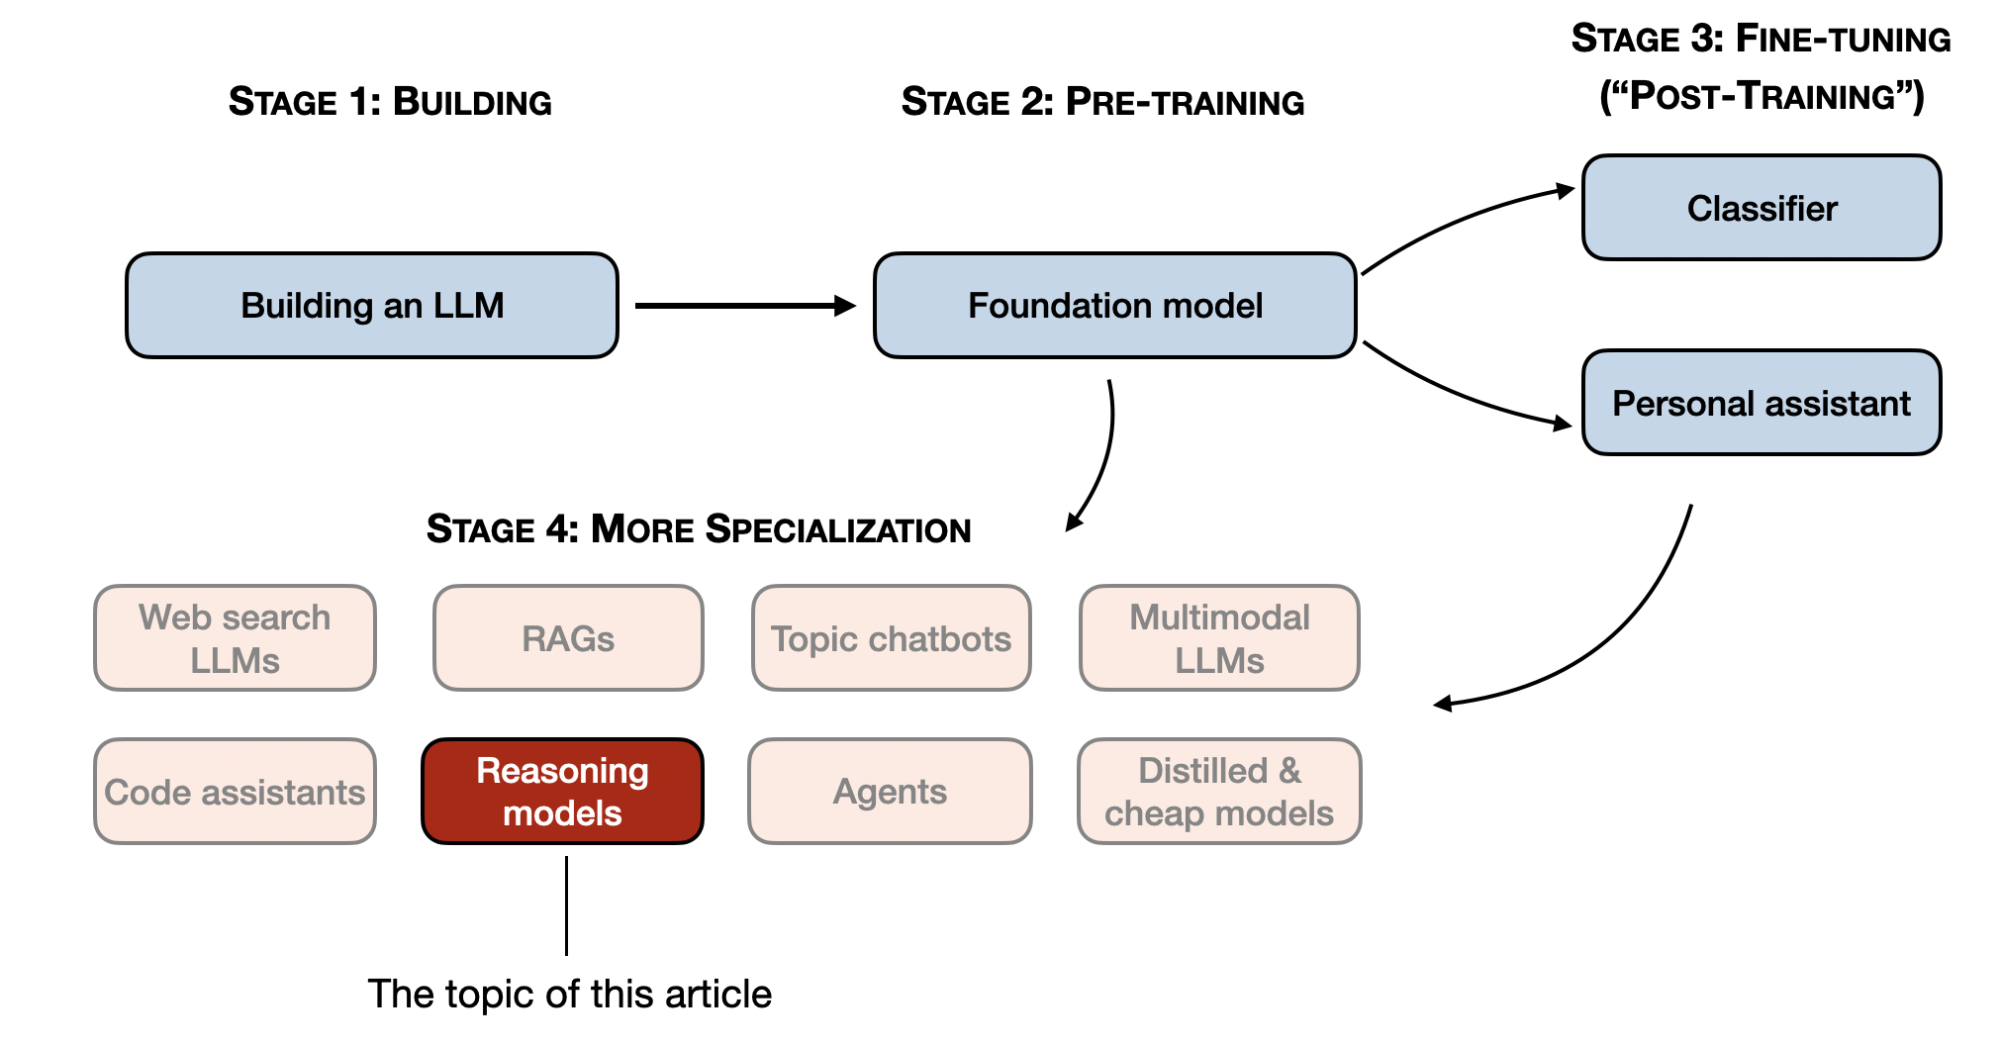
\includegraphics[width=\linewidth,keepaspectratio]{llm192}
		
		
		Stages 1-3 are the common steps to developing LLMs. Stage 4 specializes LLMs for specific use 
		cases.
		
		
		{\tiny (Ref: Understanding Reasoning LLMs - Sebastian Raschka)}
		
		\end{center}
		
\end{frame}
		
%%%%%%%%%%%%%%%%%%%%%%%%%%%%%%%%%%%%%%%%%%%%%%%%%%%%%%%%%%%%%%%%%%%%%%%%%%%%%%%%%%
\begin{frame}[fragile]\frametitle{Background: Human Reasoning}
\begin{itemize}
  \item Humans naturally think deeply to navigate life.
  \item Reasoning involves process of answering which requires many multi-step thoughts.
  \item Example: Choosing a cake requires memory, judgment, preference checks.
  \item We consider past experiences and future expectations.
  \item Reasoning helps handle ambiguity and subjective decisions.
  \item Not all questions require deep thought.
  \item Quick factual questions can be answered instantly.
  \item This contrast helps define different types of reasoning.
  \item AI is supposed to mimic Human Intelligence, but it does not. It does not `think' like Humans but `answers' like Humans, at least the ChatGPT 3.5 model.
\end{itemize}

\end{frame}

%%%%%%%%%%%%%%%%%%%%%%%%%%%%%%%%%%%%%%%%%%%%%%%%%%%%%%%%%%%%%%%%%%%%%%%%%%%%%%%%%%
\begin{frame}[fragile]\frametitle{Example: Reasoning}

		\begin{center}
		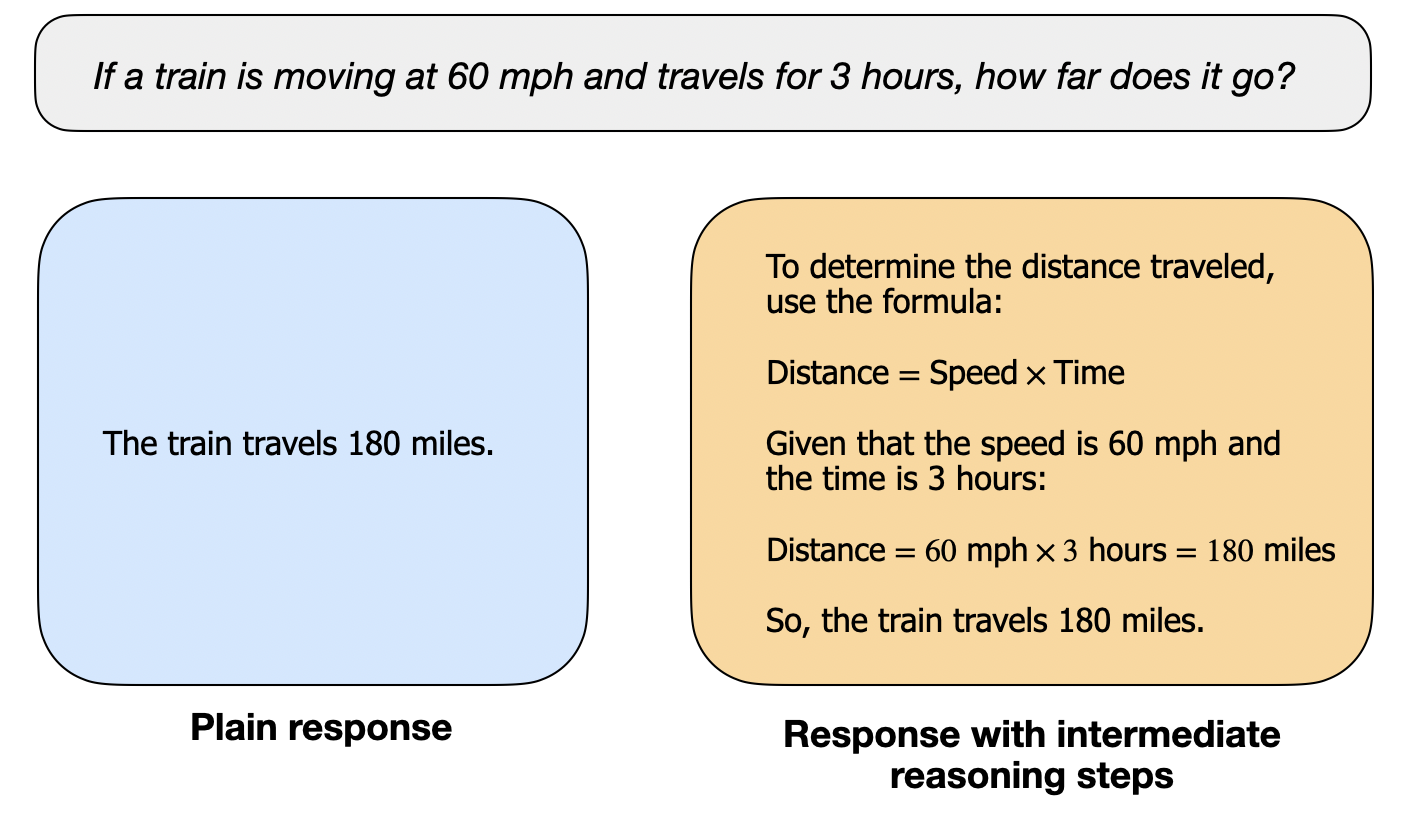
\includegraphics[width=\linewidth,keepaspectratio]{llm193}
		
		{\tiny (Ref: Understanding Reasoning LLMs - Sebastian Raschka)}
		
		\end{center}
\end{frame}


%%%%%%%%%%%%%%%%%%%%%%%%%%%%%%%%%%%%%%%%%%%%%%%%%%%%%%%%%%%%%%%%%%%%%%%%%%%%%%%%%%
\begin{frame}[fragile]\frametitle{Fast vs Slow Reasoning}

\begin{columns}
    \begin{column}[T]{0.6\linewidth}
		\begin{itemize}
		  \item Two types: Fast (System 1) and Slow (System 2).
		  \item Fast reasoning is instinctive and automatic.
		  \item Example: Answering ``What is the capital of India?''
		  \item Slow reasoning is deliberate and effortful.
		  \item Example: Choosing a movie to watch.
		  \item System 1 is fast but error-prone.
		  \item System 2 is slower but more accurate.
		  \item Based on Daniel Kahneman's theory in ``Thinking, Fast and Slow''.
		  \item Useful framework for evaluating human and machine reasoning.
		\end{itemize}

    \end{column}
    \begin{column}[T]{0.4\linewidth}
		\begin{center}
		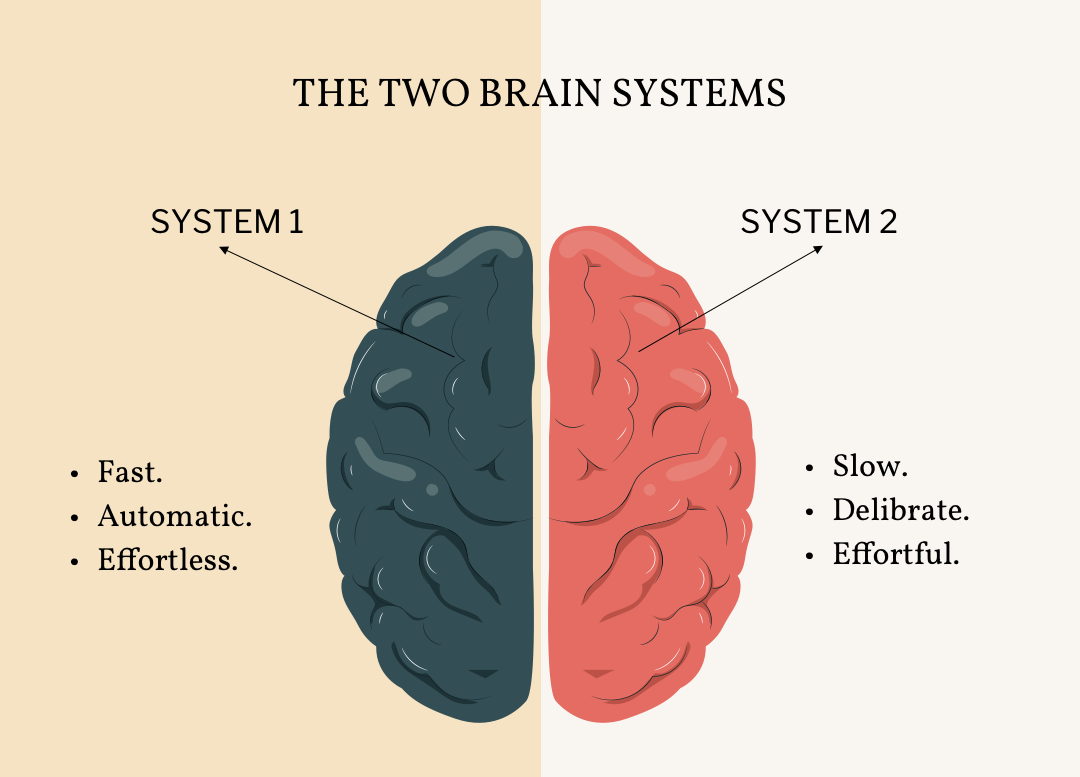
\includegraphics[width=0.8\linewidth,keepaspectratio]{llm144}
		
		{\tiny (Ref: What are Large Reasoning Models? - Vizuara AI)}
		
		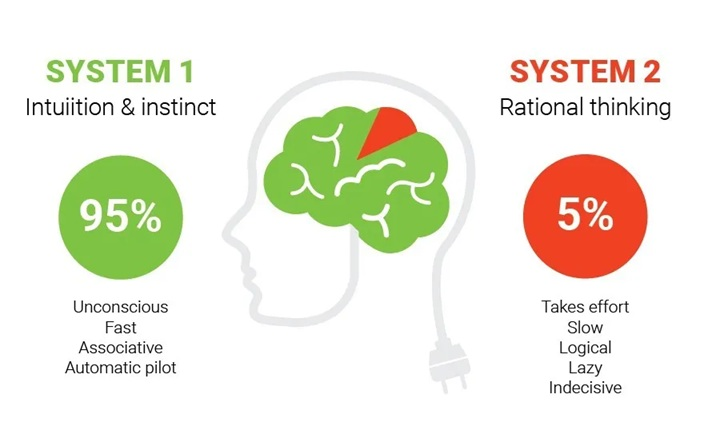
\includegraphics[width=0.8\linewidth,keepaspectratio]{llm189}
		
		{\tiny (Ref: Bridging Generative Models and System 1 with System 2 - Nguyen Ha Thanh)}
		
		\end{center}
    \end{column}
  \end{columns}
 
\end{frame}

%%%%%%%%%%%%%%%%%%%%%%%%%%%%%%%%%%%%%%%%%%%%%%%%%%%%%%%%%%%%%%%%%%%%%%%%%%%%%%%%%%
\begin{frame}[fragile]\frametitle{Can LLMs Reason?}


\begin{columns}
    \begin{column}[T]{0.5\linewidth}
		\begin{itemize}
		  \item LLMs are trained to imitate, not reason. (True for ChatGPT 3.5 and likes)
		  \item Early LLMs excelled at fast (System 1) tasks.
		  \item Poor performance on complex (System 2) tasks.
		  \item Often failed simple reasoning like spelling or logic.
		  \item Operate as pattern matchers over vast text corpora.
		  \item Answers based on likelihood, not understanding.
		  \item ChatGPT amazed users but still lacked true reasoning.
		  \item Triggered interest in reasoning-capable AI models.
		\end{itemize}

    \end{column}
    \begin{column}[T]{0.5\linewidth}
		\begin{center}
		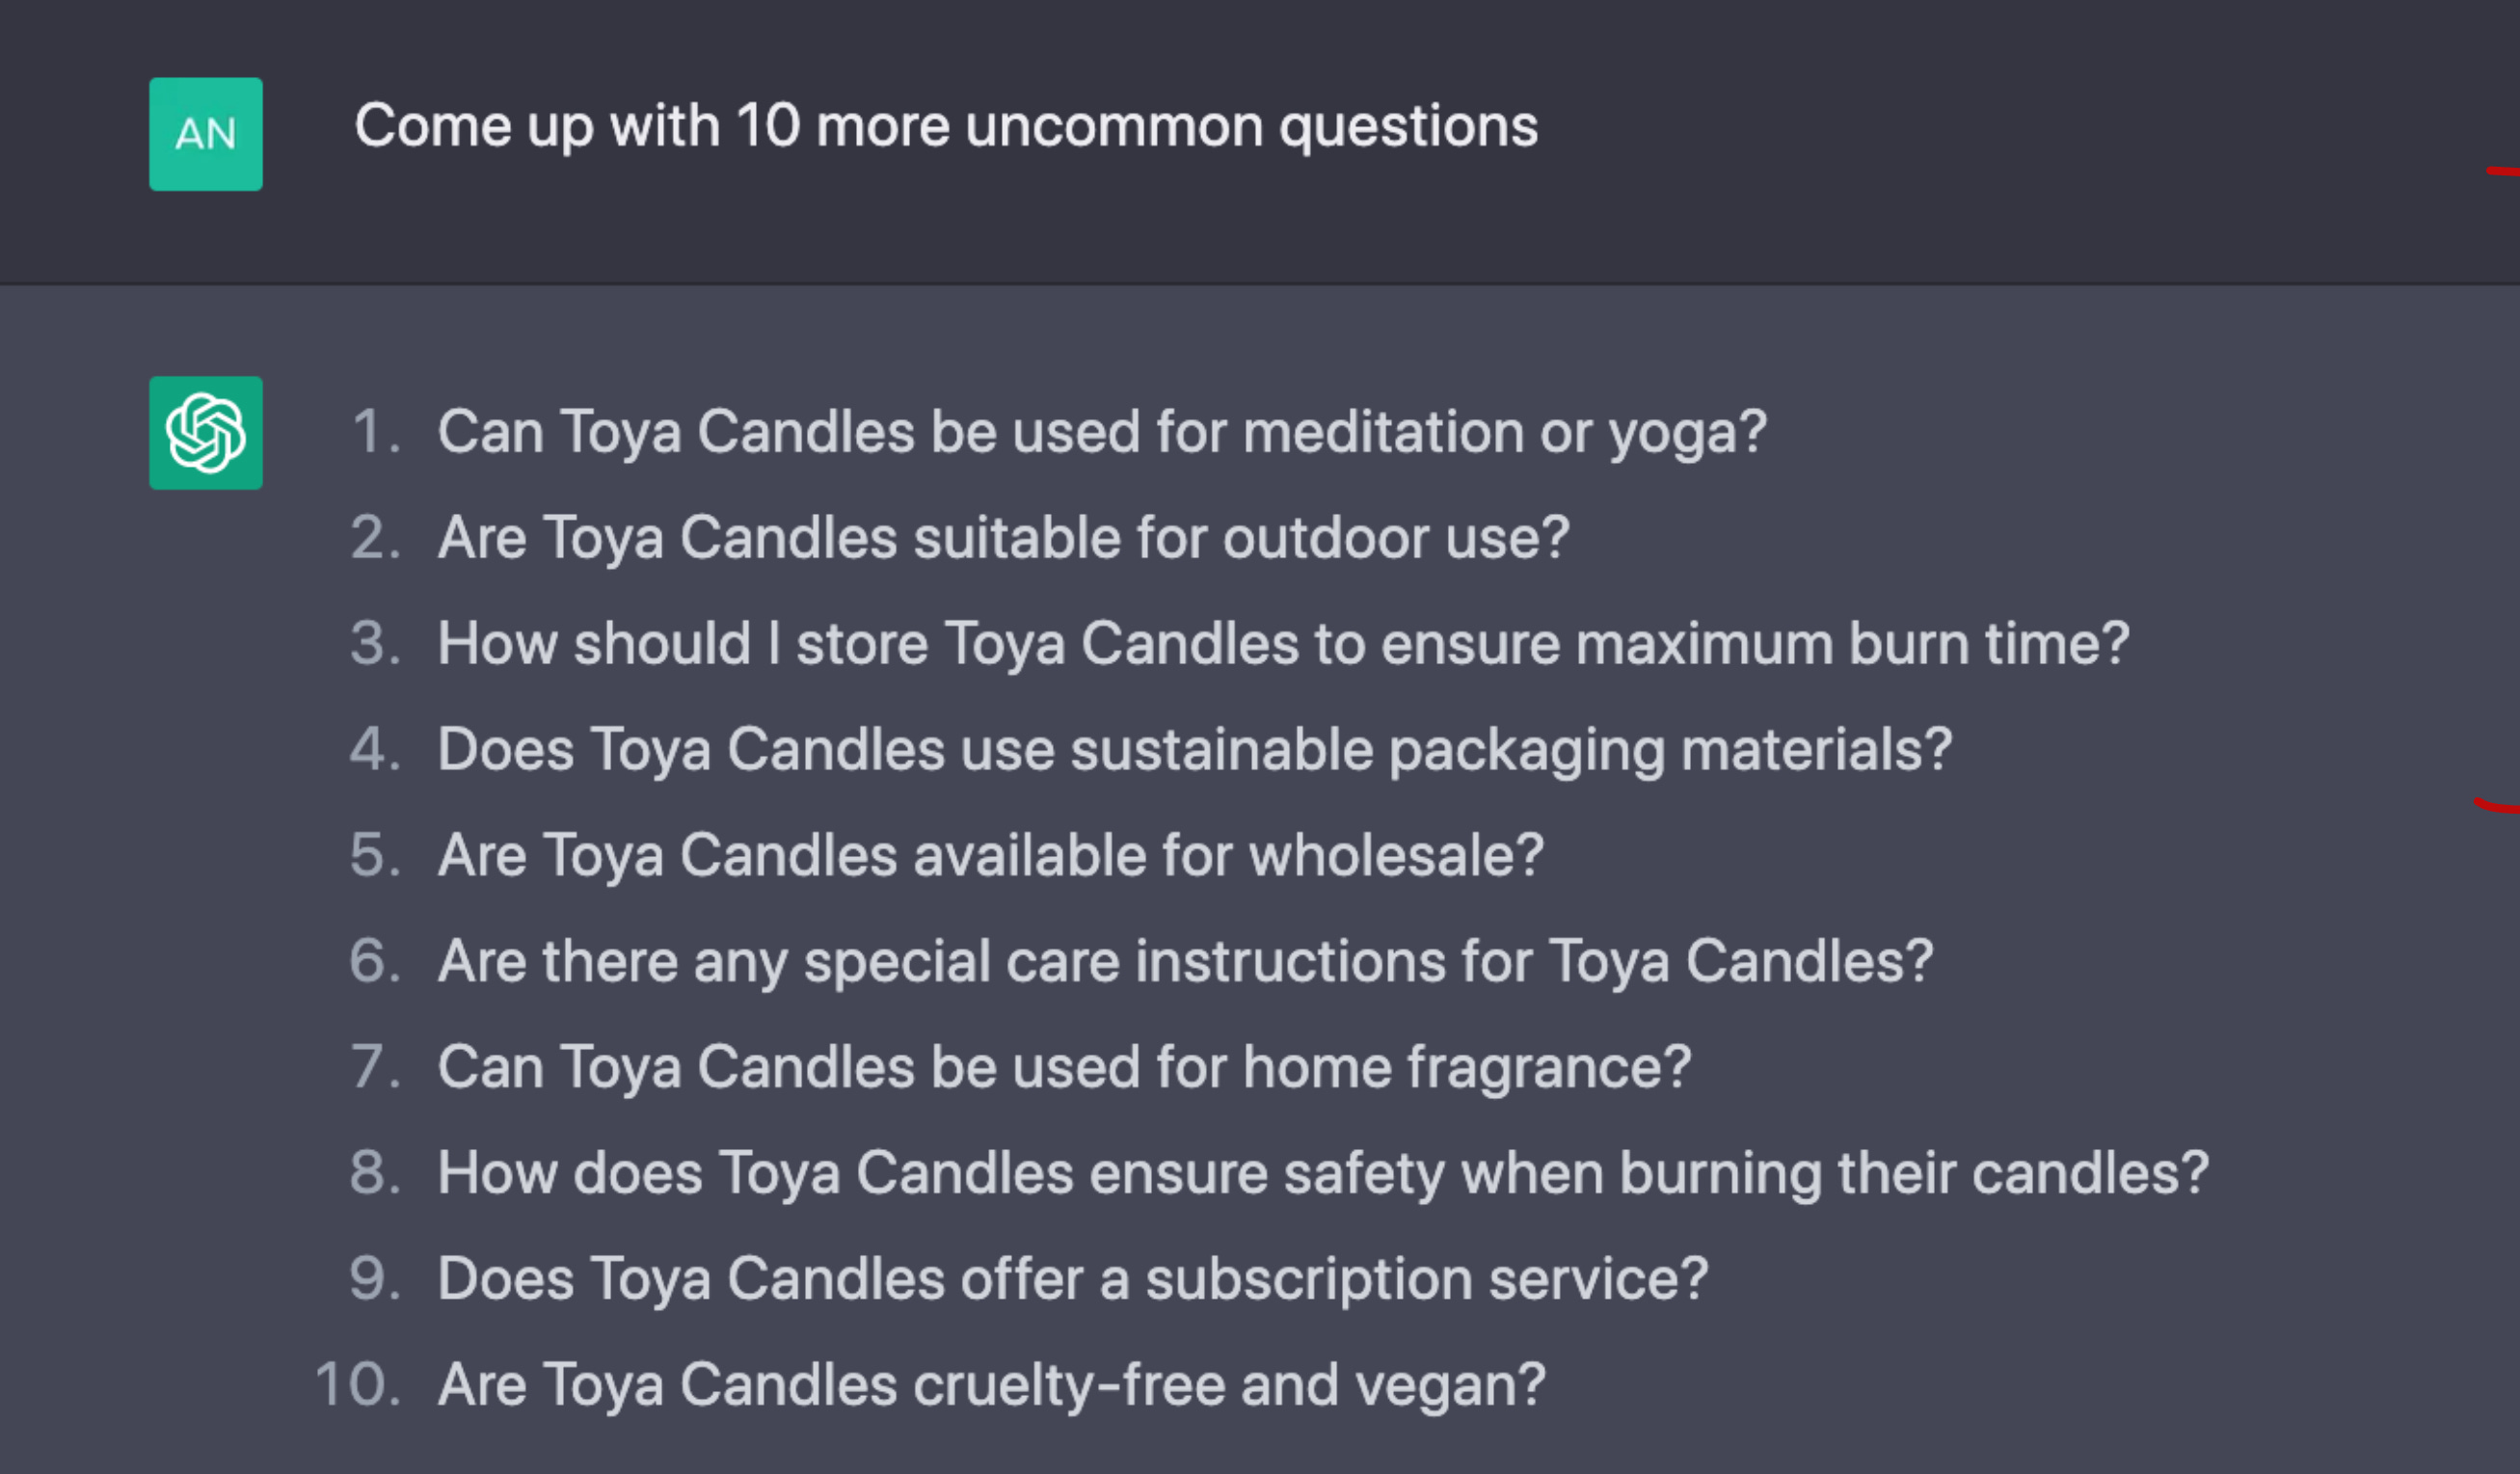
\includegraphics[width=0.7\linewidth,keepaspectratio]{llm145}

		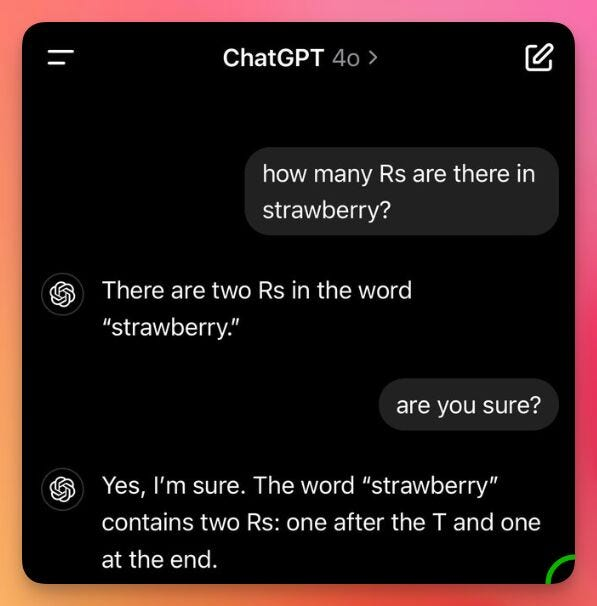
\includegraphics[width=0.7\linewidth,keepaspectratio]{llm146}
		
		{\tiny (Ref: What are Large Reasoning Models? - Vizuara AI)}
		
		\end{center}
    \end{column}
  \end{columns}
	

\end{frame}

%%%%%%%%%%%%%%%%%%%%%%%%%%%%%%%%%%%%%%%%%%%%%%%%%%%%%%%%%%%%%%%%%%%%%%%%%%%%%%%%%%
\begin{frame}[fragile]\frametitle{The Quest for Reasoning Models}

% \begin{columns}
    % \begin{column}[T]{0.6\linewidth}
		\begin{itemize}
		  \item OpenAI’s o1 (2024) showed signs of reasoning.
		  \item Response delay hinted at internal deliberation.
		  \item No open-source insight into o1’s mechanism.
		  \item DeepSeek-R1 (2025) rivaled o1’s performance.
		  \item DeepSeek-R1 was fully open-source, was trained by pure Reinforcement Learning.
		  \item Revealed blueprint for reasoning-capable LLMs.
		  \item Introduced 4 key ingredients in model design.
		  \item Marked major leap in human-like AI reasoning.
		\end{itemize}

    % \end{column}
    % \begin{column}[T]{0.4\linewidth}
		\begin{center}
		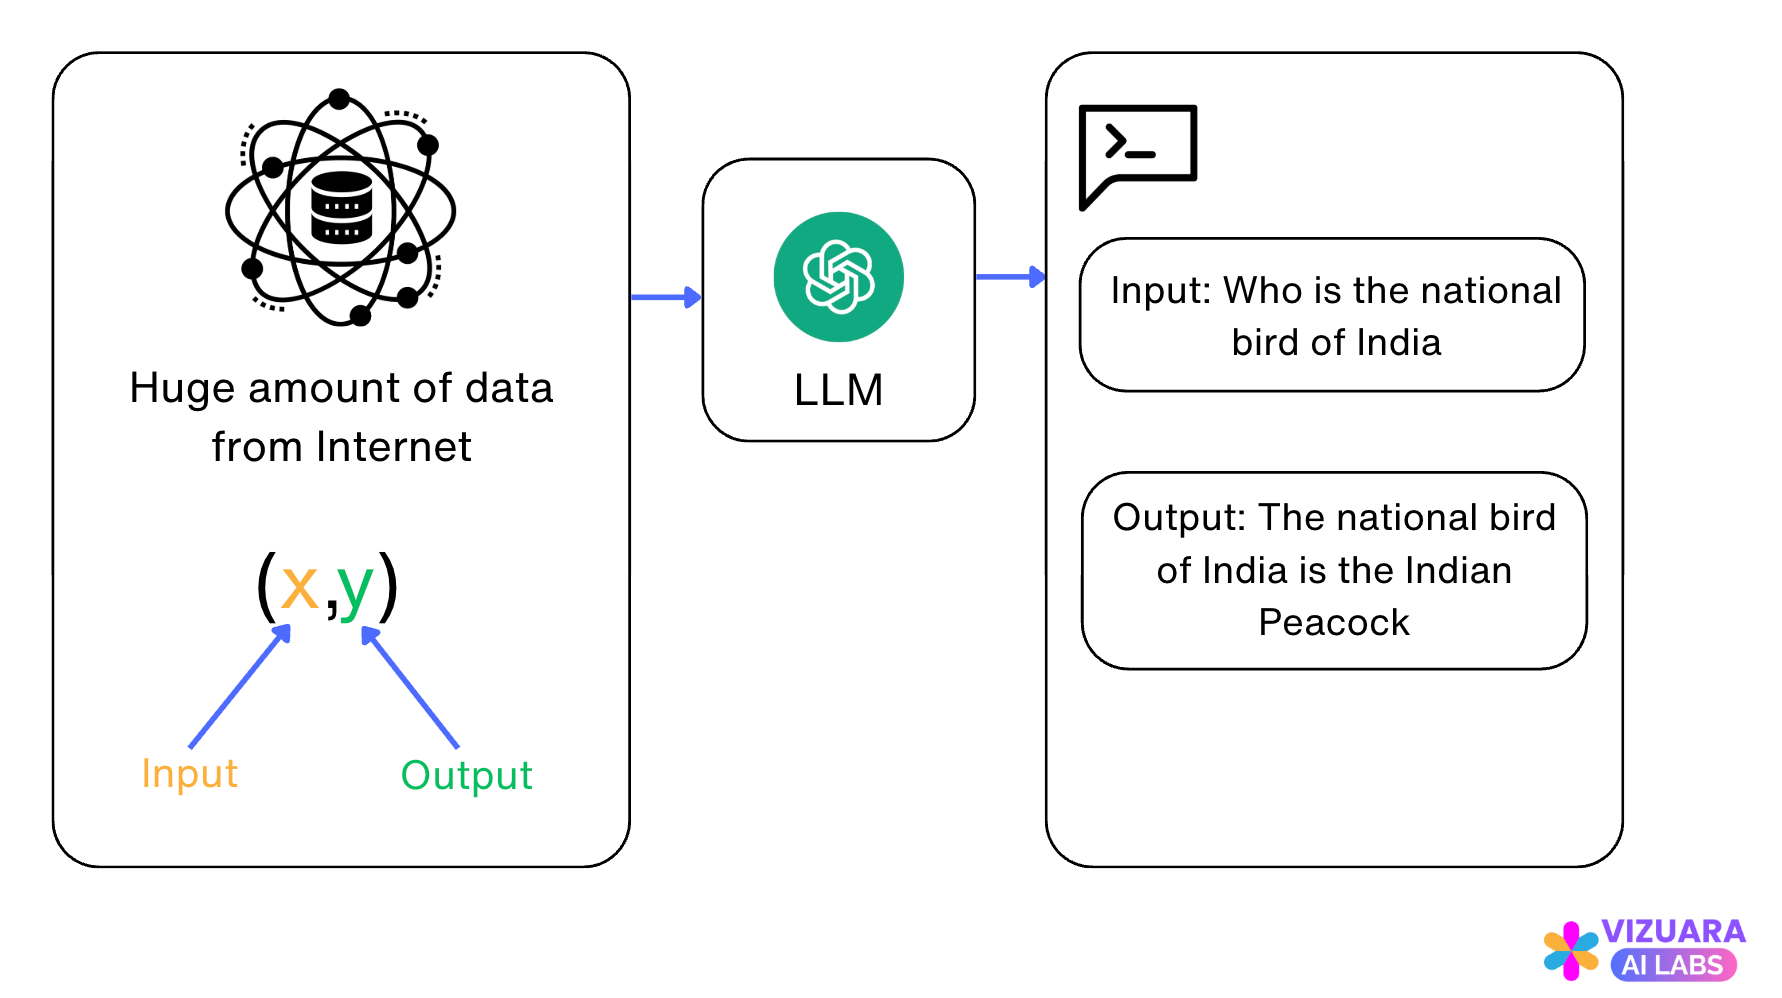
\includegraphics[width=0.5\linewidth,keepaspectratio]{llm147}
		
		{\tiny (Ref: What are Large Reasoning Models? - Vizuara AI)}
		
		\end{center}
    % \end{column}
  % \end{columns}

\end{frame}

%%%%%%%%%%%%%%%%%%%%%%%%%%%%%%%%%%%%%%%%%%%%%%%%%%%%%%%%%%%%%%%%%%%%%%%%%%%%%%%%%%
\begin{frame}[fragile]\frametitle{Closed 'o1' but Open 'R1'}

\begin{columns}
    \begin{column}[T]{0.5\linewidth}
		\begin{center}
		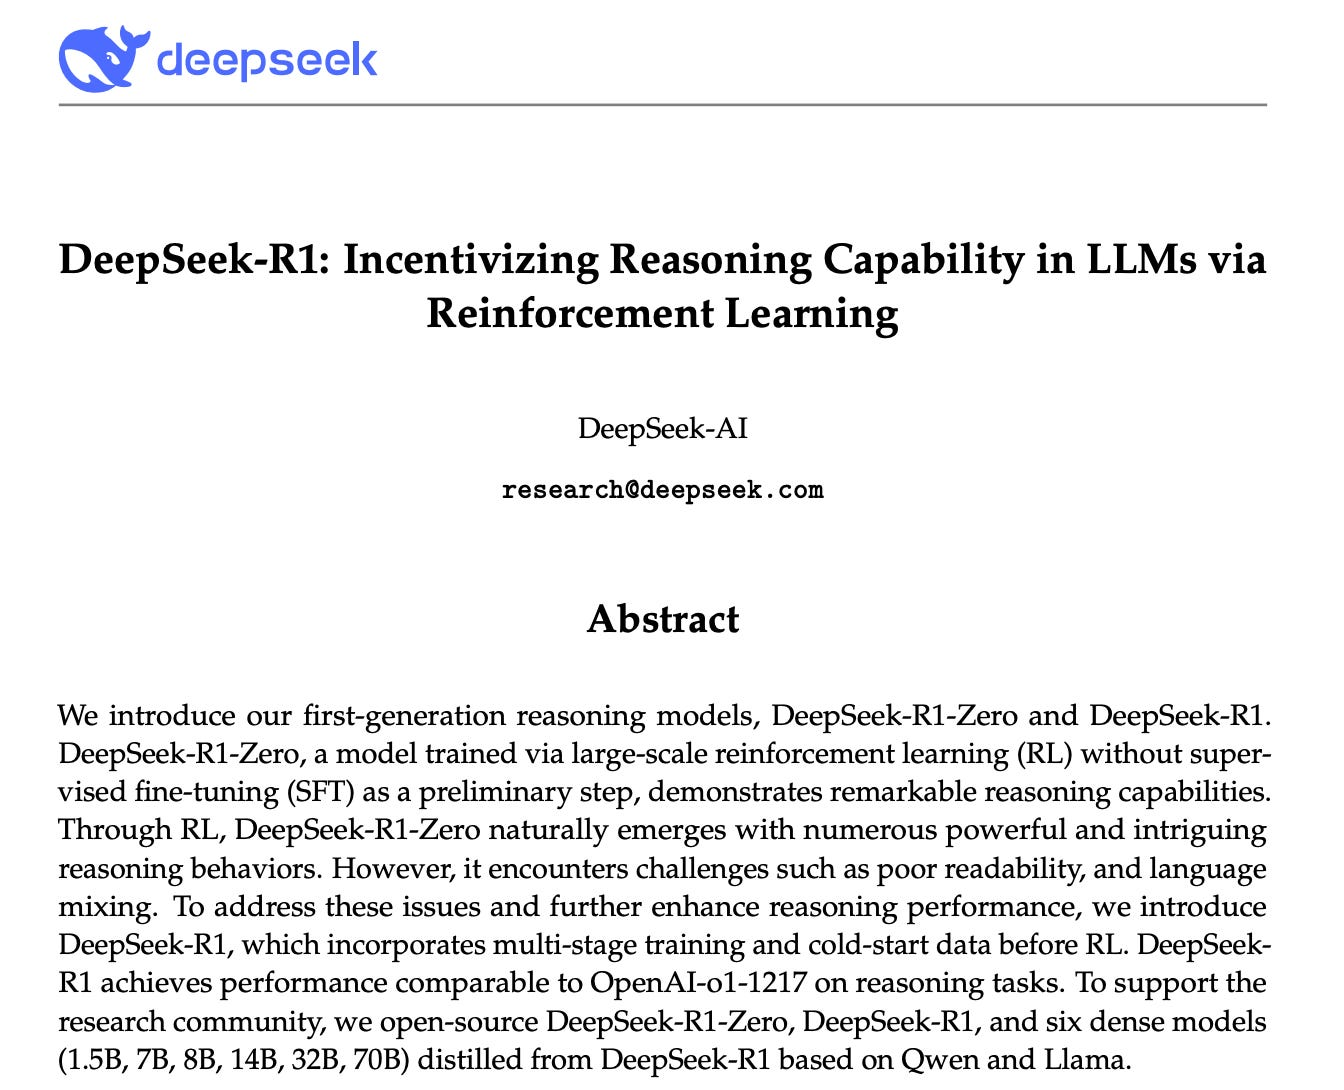
\includegraphics[width=\linewidth,keepaspectratio]{llm148}		
		\end{center}
    \end{column}
    \begin{column}[T]{0.5\linewidth}	
		\begin{center}
		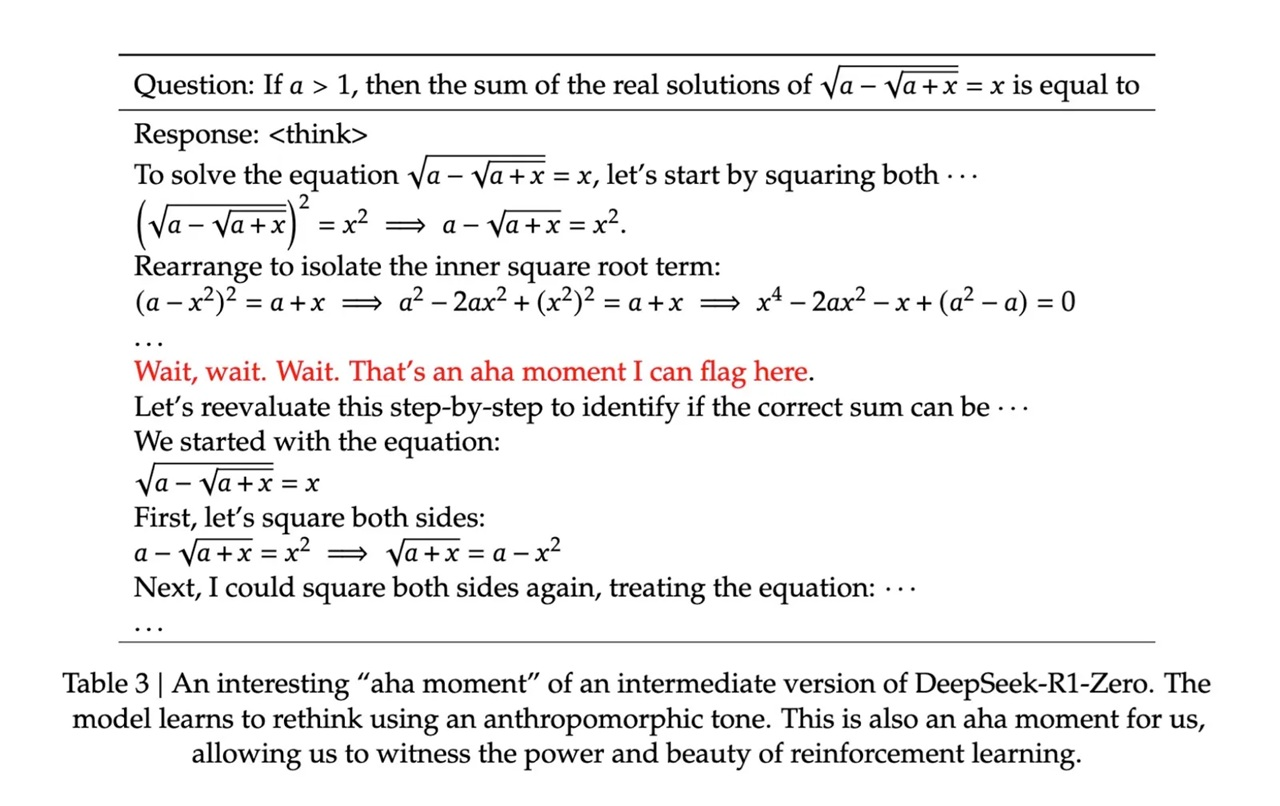
\includegraphics[width=\linewidth,keepaspectratio]{llm190}
		\end{center}	
    \end{column}
  \end{columns}


It did not just spit the most predicable answer but 'thought' and 'realized'!!
\end{frame}

%%%%%%%%%%%%%%%%%%%%%%%%%%%%%%%%%%%%%%%%%%%%%%%%%%%%%%%%%%%%%%%%%%%%%%%%%%%%%%%%%%
\begin{frame}[fragile]\frametitle{LLM vs LRM}

		\begin{center}
		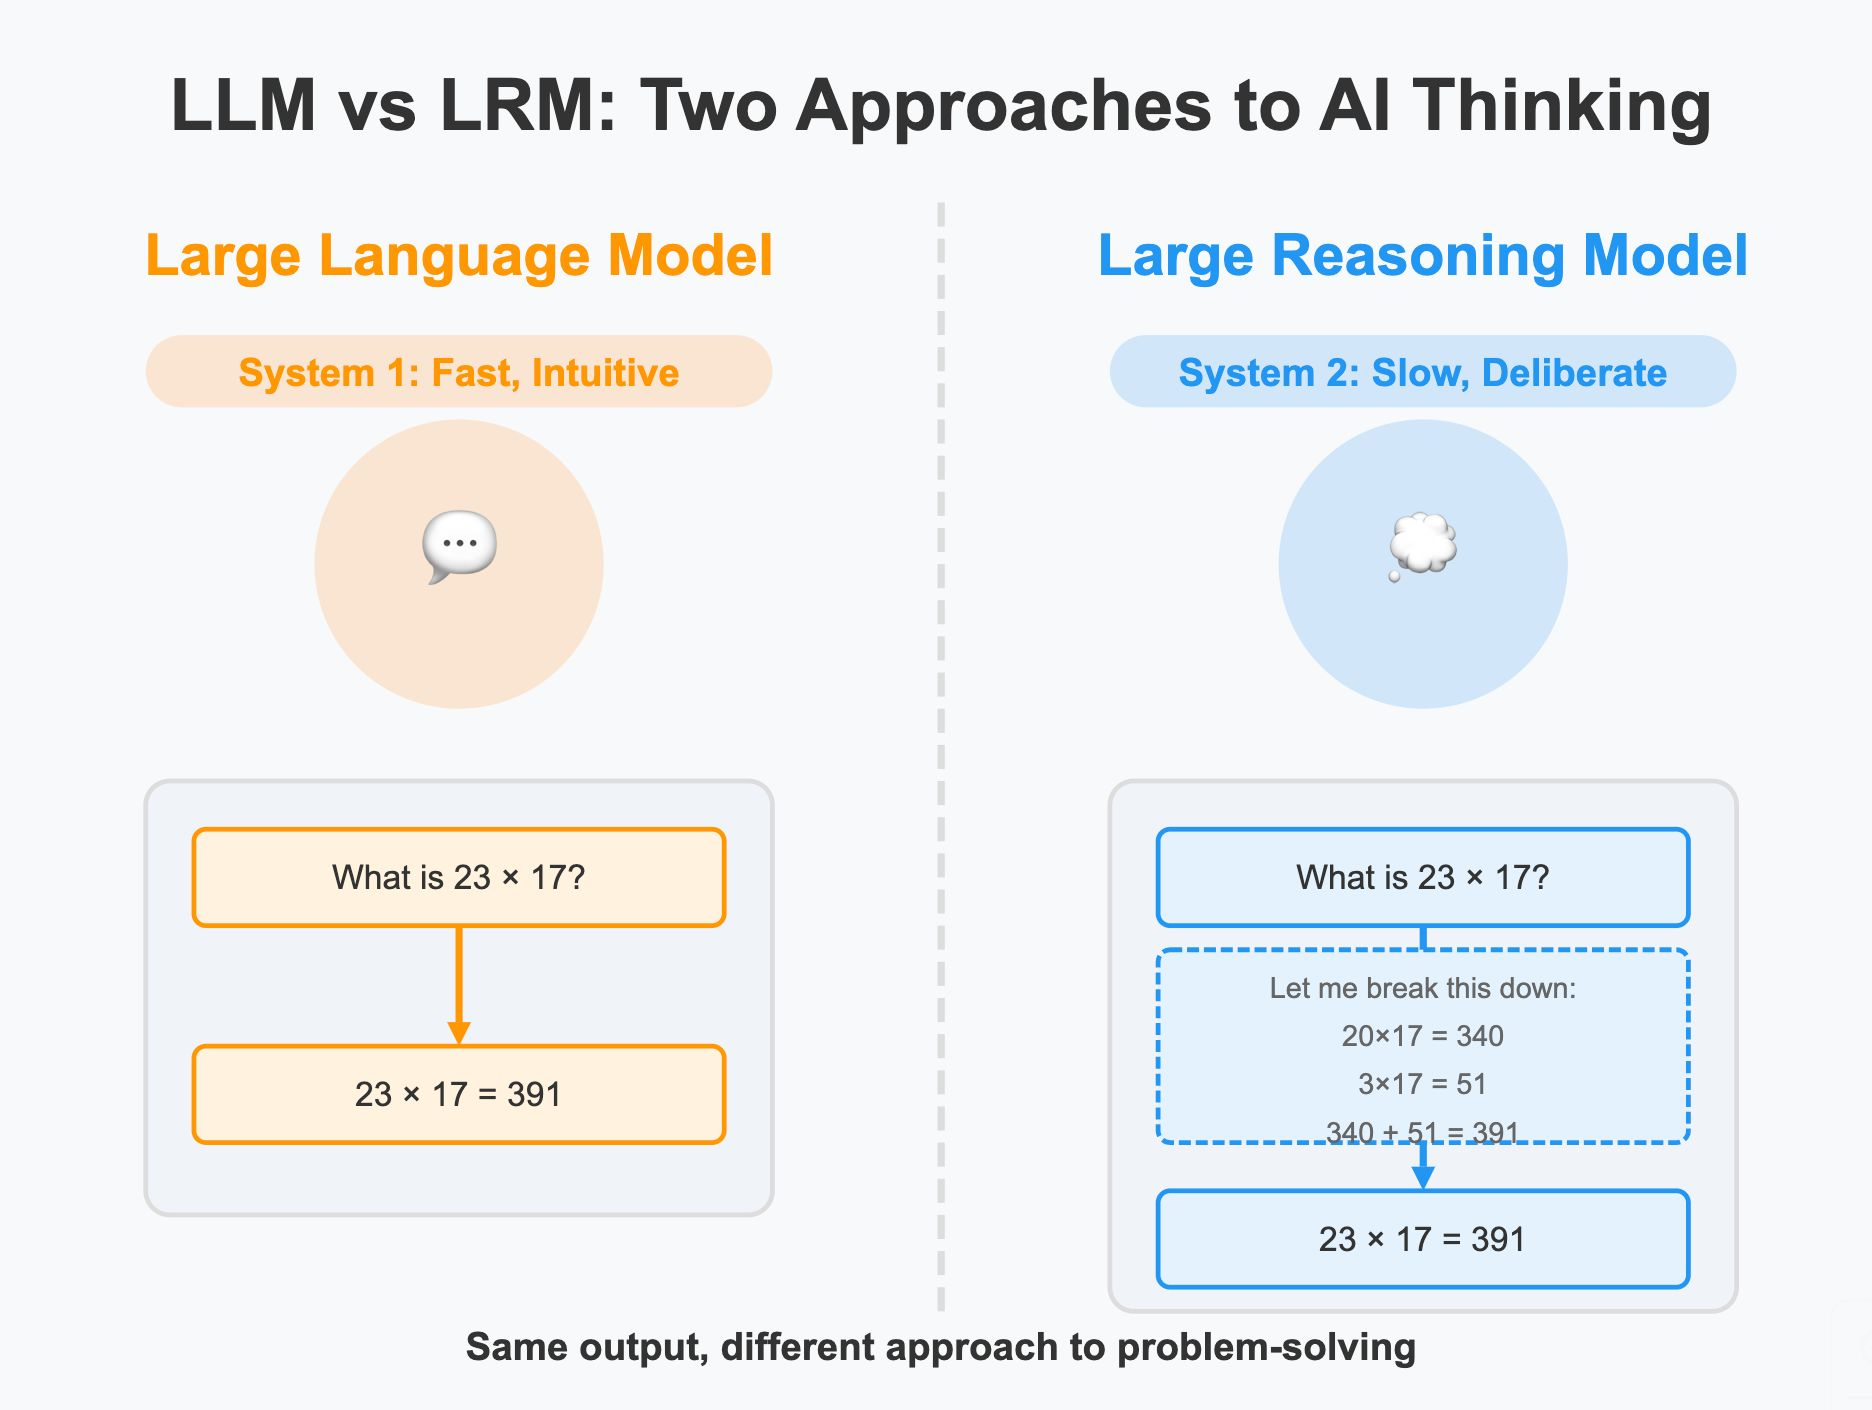
\includegraphics[width=0.7\linewidth,keepaspectratio]{llm191}
		
		{\tiny (Ref: LinkedIn post by Riley Thomas)}

		\end{center}	

\end{frame}

%%%%%%%%%%%%%%%%%%%%%%%%%%%%%%%%%%%%%%%%%%%%%%%%%%%%%%%%%%%%%%%%%%%%%%%%%%%%%%%%%%
\begin{frame}[fragile]\frametitle{Overview }

4 Modules/Ingredient: 

		\begin{itemize}
		  \item Ingredient 1: Inference-Time Compute Scaling
		  \item Ingredient 2: Pure Reinforcement Learning
		  \item Ingredient 3: Supervised Fine-Tuning + RL
		  \item Ingredient 4: Distillation
		\end{itemize}
\end{frame}

%%%%%%%%%%%%%%%%%%%%%%%%%%%%%%%%%%%%%%%%%%%%%%%%%%%%%%%%%%%%%%%%%%%%%%%%%%%%%%%%%%
\begin{frame}[fragile]\frametitle{Ingredient 1: Inference-Time Compute Scaling}

\begin{columns}
    \begin{column}[T]{0.8\linewidth}
		\begin{itemize}
		  \item Humans give better answers when they think for more time. Why? because thinking step by step leads to a correct answer
		  \item For LLM, we do not change anything, but just give more inference time/compute → better reasoning/answer, via asking to generate step-by-step thoughts.
		  \item Prompting techniques: ``Let’s think step by step'', induces chains of thought.
		  \item Encourages reflection before final output.
		  \item Supports System 2-like thinking in LLMs.
		  \item Example: Sudoku. Cannot just start putting numbers. Need longer reasoning chain.
		  
		\end{itemize}

    \end{column}
    \begin{column}[T]{0.2\linewidth}
		\begin{center}
		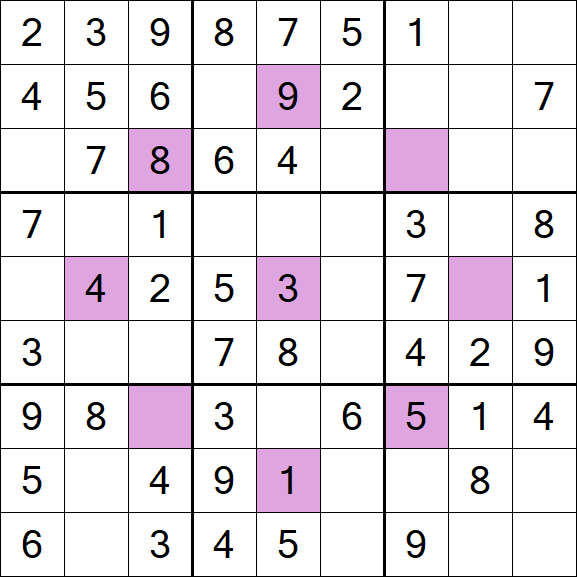
\includegraphics[width=\linewidth,keepaspectratio]{llm149}
		
		{\tiny (Ref: What are Large Reasoning Models? - Vizuara AI)}
		
		\end{center}
    \end{column}
  \end{columns}


\end{frame}

%%%%%%%%%%%%%%%%%%%%%%%%%%%%%%%%%%%%%%%%%%%%%%%%%%%%%%%%%%%%%%%%%%%%%%%%%%%%%%%%%%
\begin{frame}[fragile]\frametitle{More Tokens}

Token usage increases with thought depth.

\begin{columns}
    \begin{column}[T]{0.5\linewidth}
		\begin{center}
		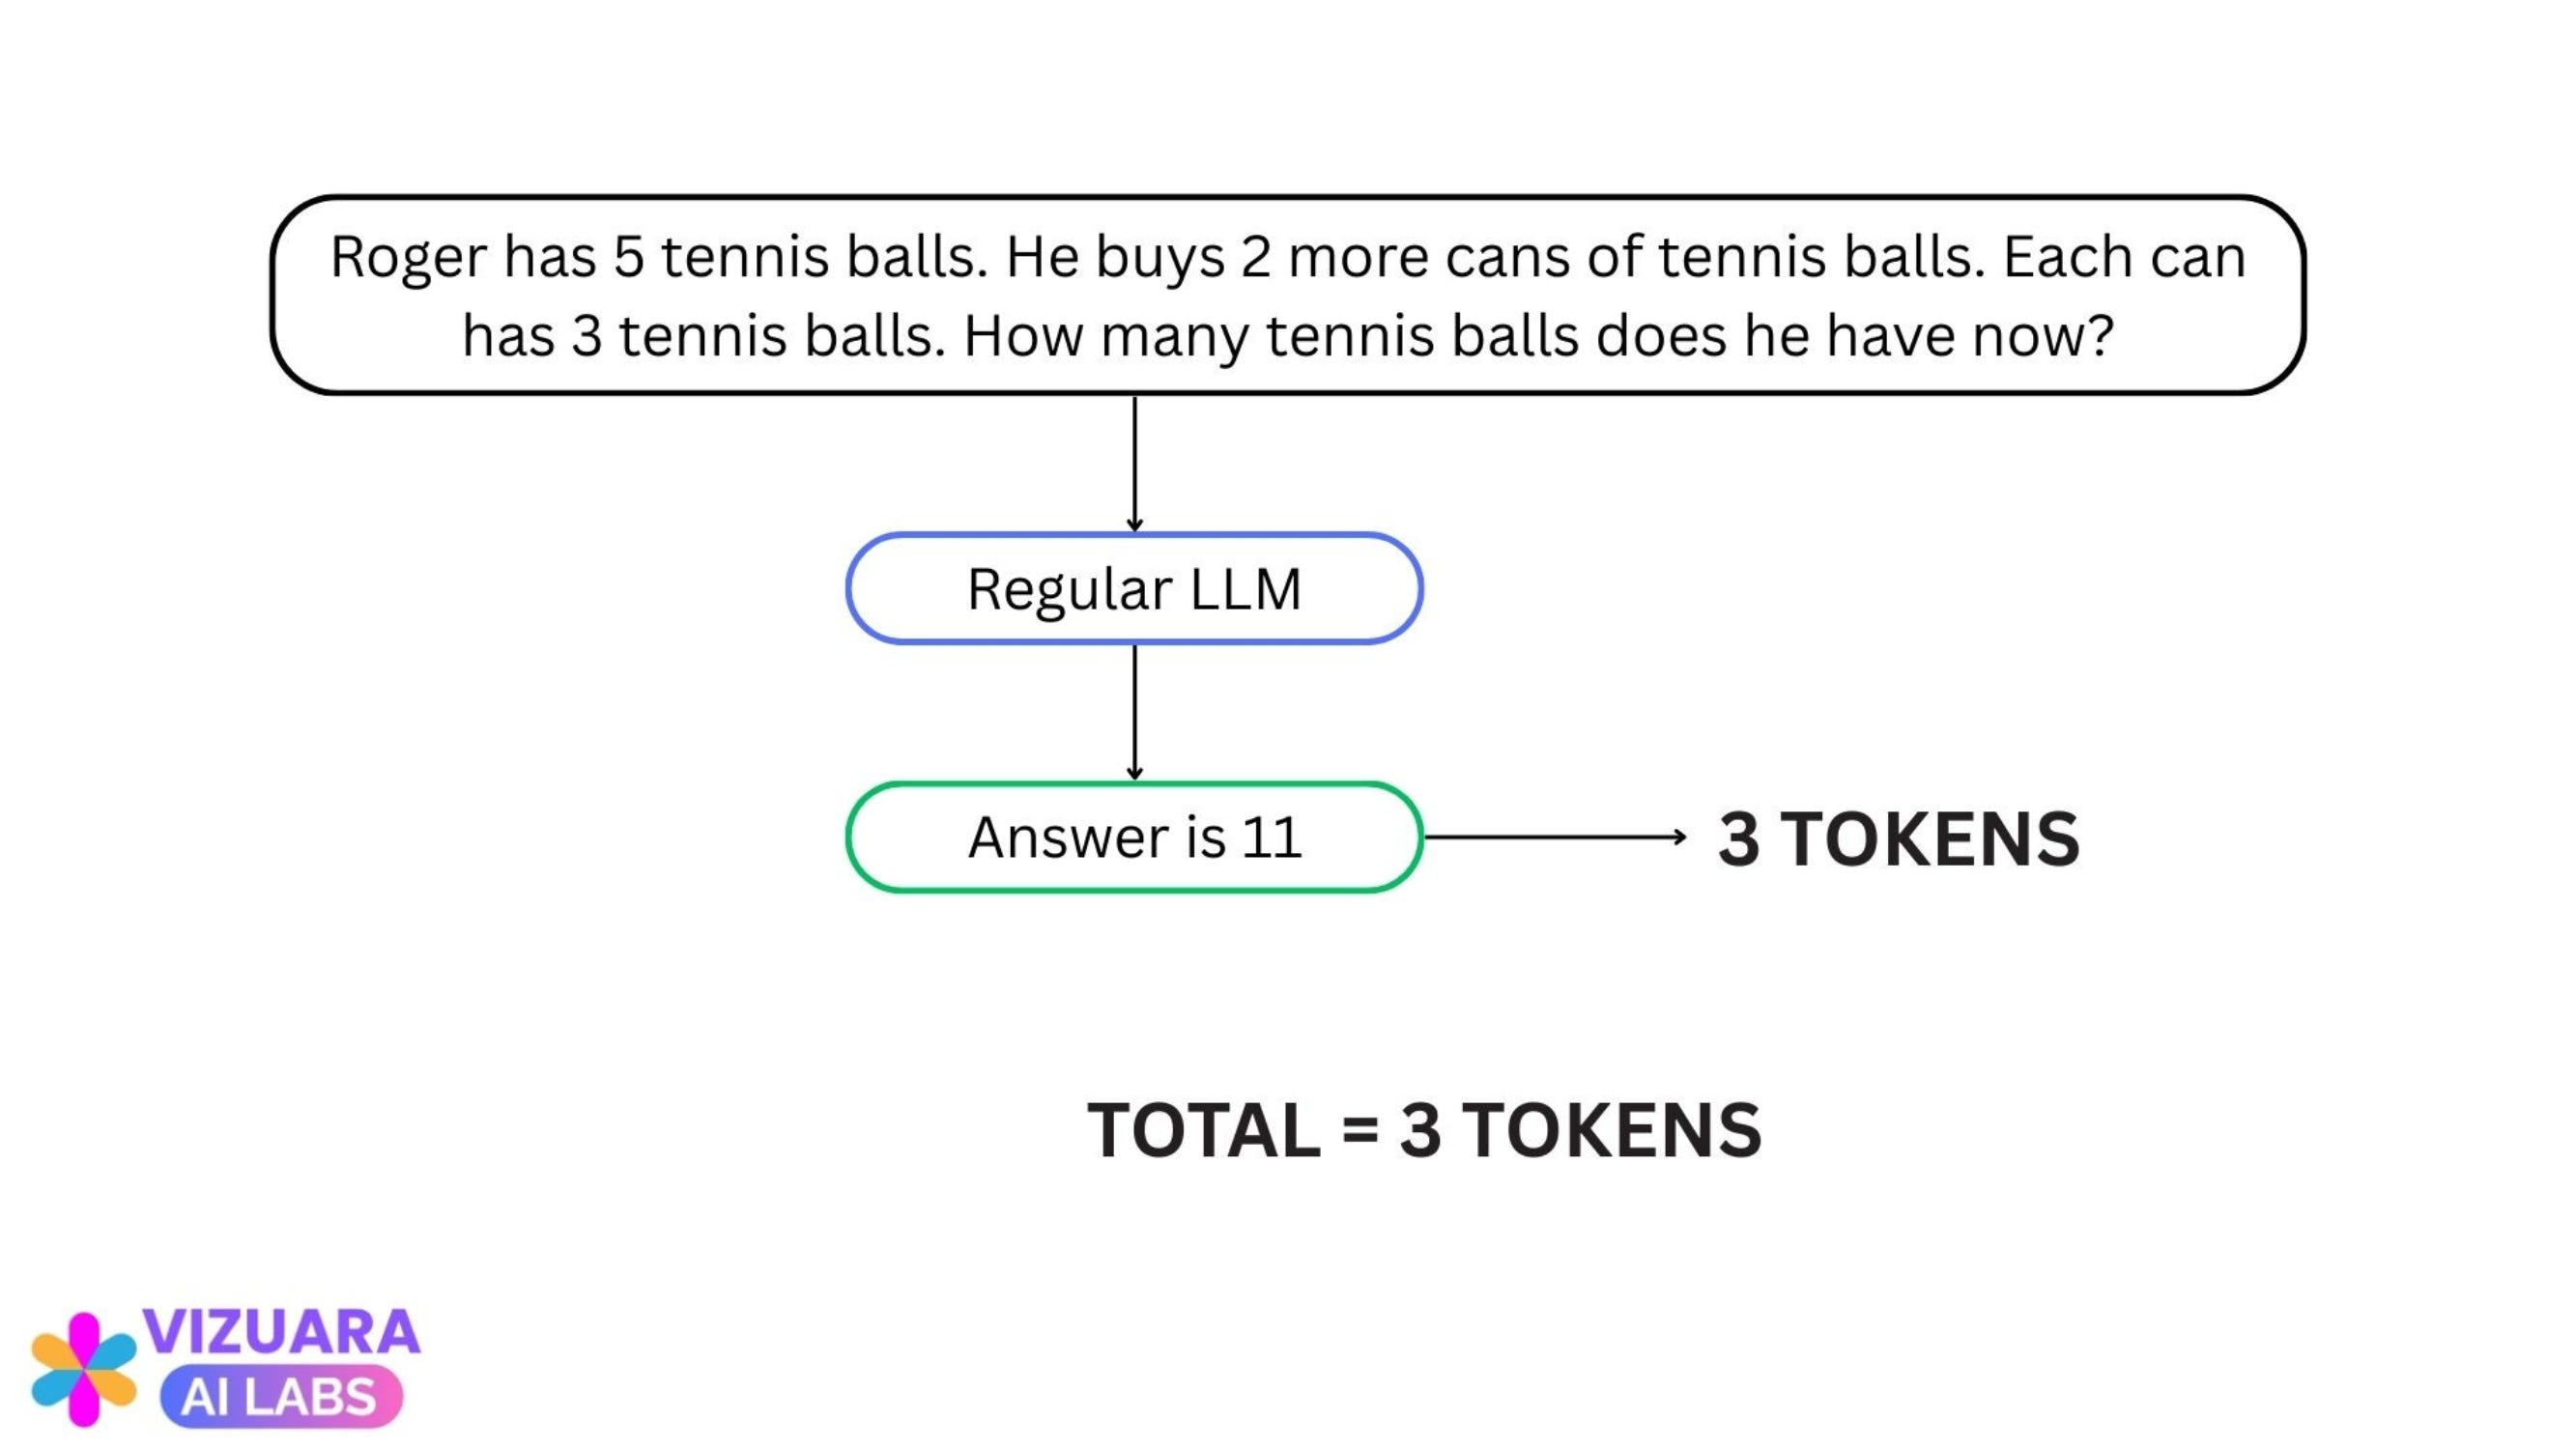
\includegraphics[width=\linewidth,keepaspectratio]{llm150}
		\end{center}

    \end{column}
    \begin{column}[T]{0.5\linewidth}
		\begin{center}
		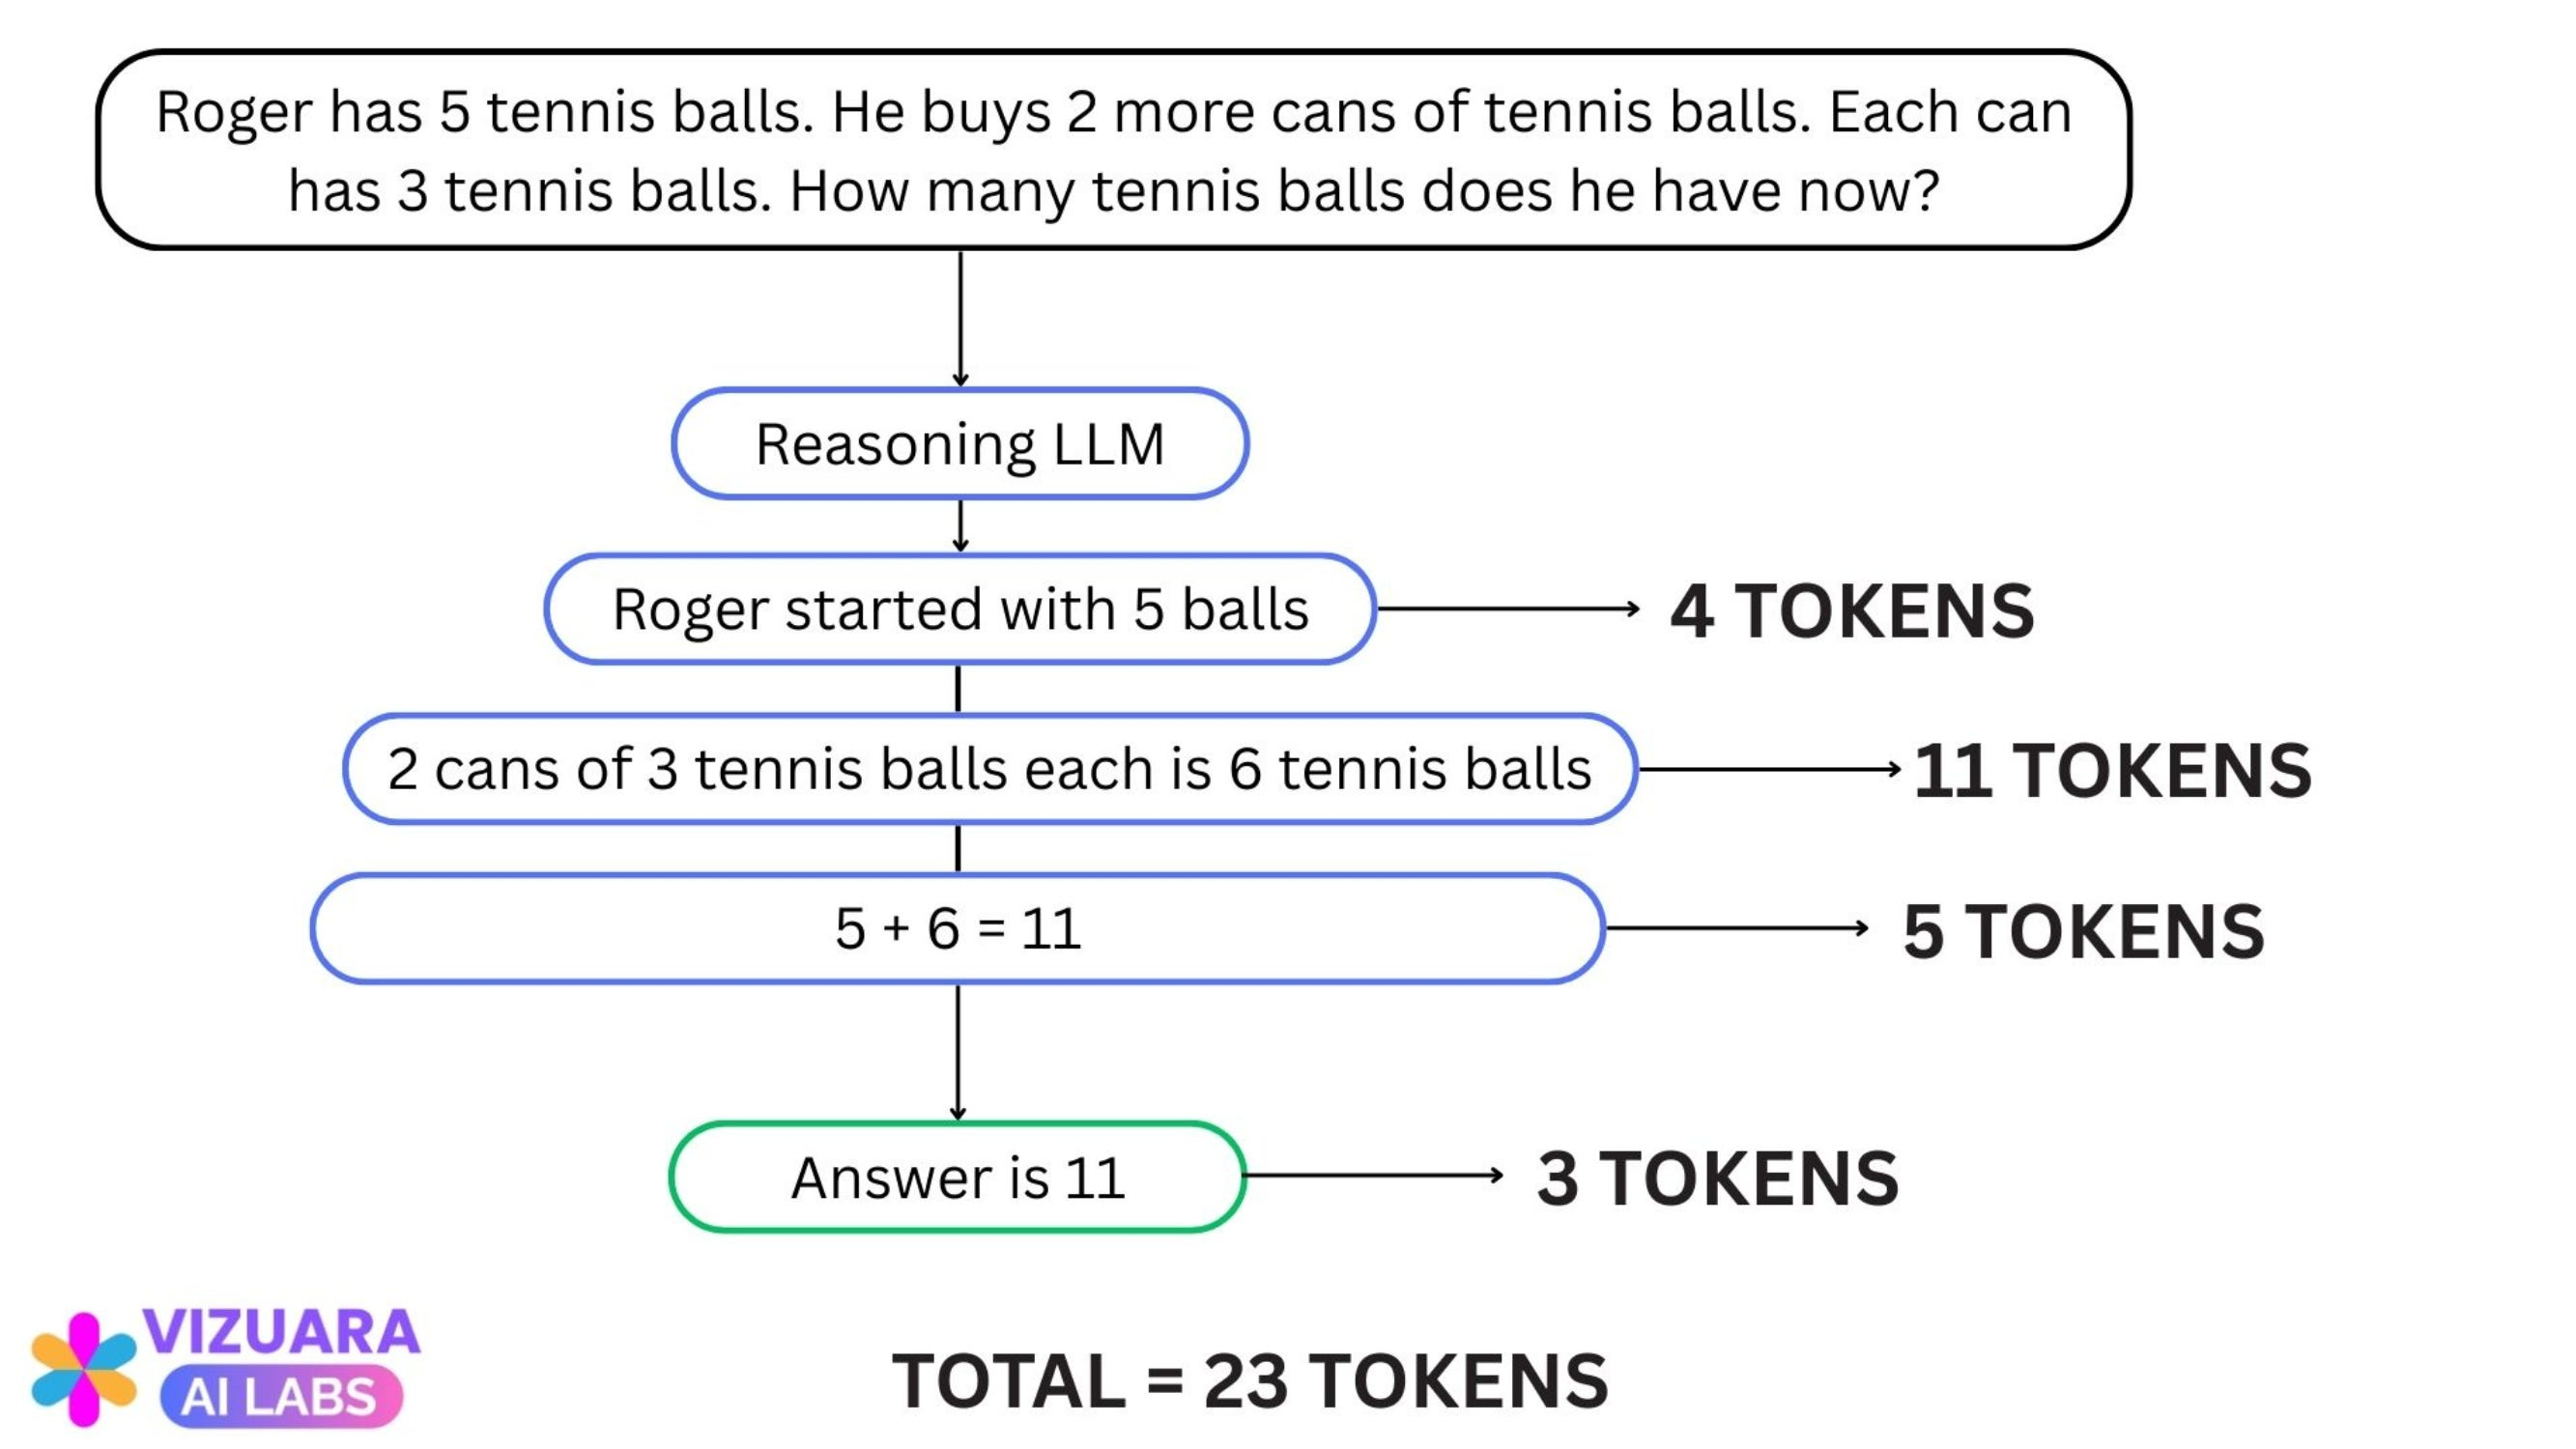
\includegraphics[width=\linewidth,keepaspectratio]{llm151}
		\end{center}
    \end{column}
  \end{columns}
  

{\tiny (Ref: What are Large Reasoning Models? - Vizuara AI)}

\end{frame}

%%%%%%%%%%%%%%%%%%%%%%%%%%%%%%%%%%%%%%%%%%%%%%%%%%%%%%%%%%%%%%%%%%%%%%%%%%%%%%%%%%
\begin{frame}[fragile]\frametitle{Train and Test}


\begin{columns}
    \begin{column}[T]{0.5\linewidth}
		\begin{center}
		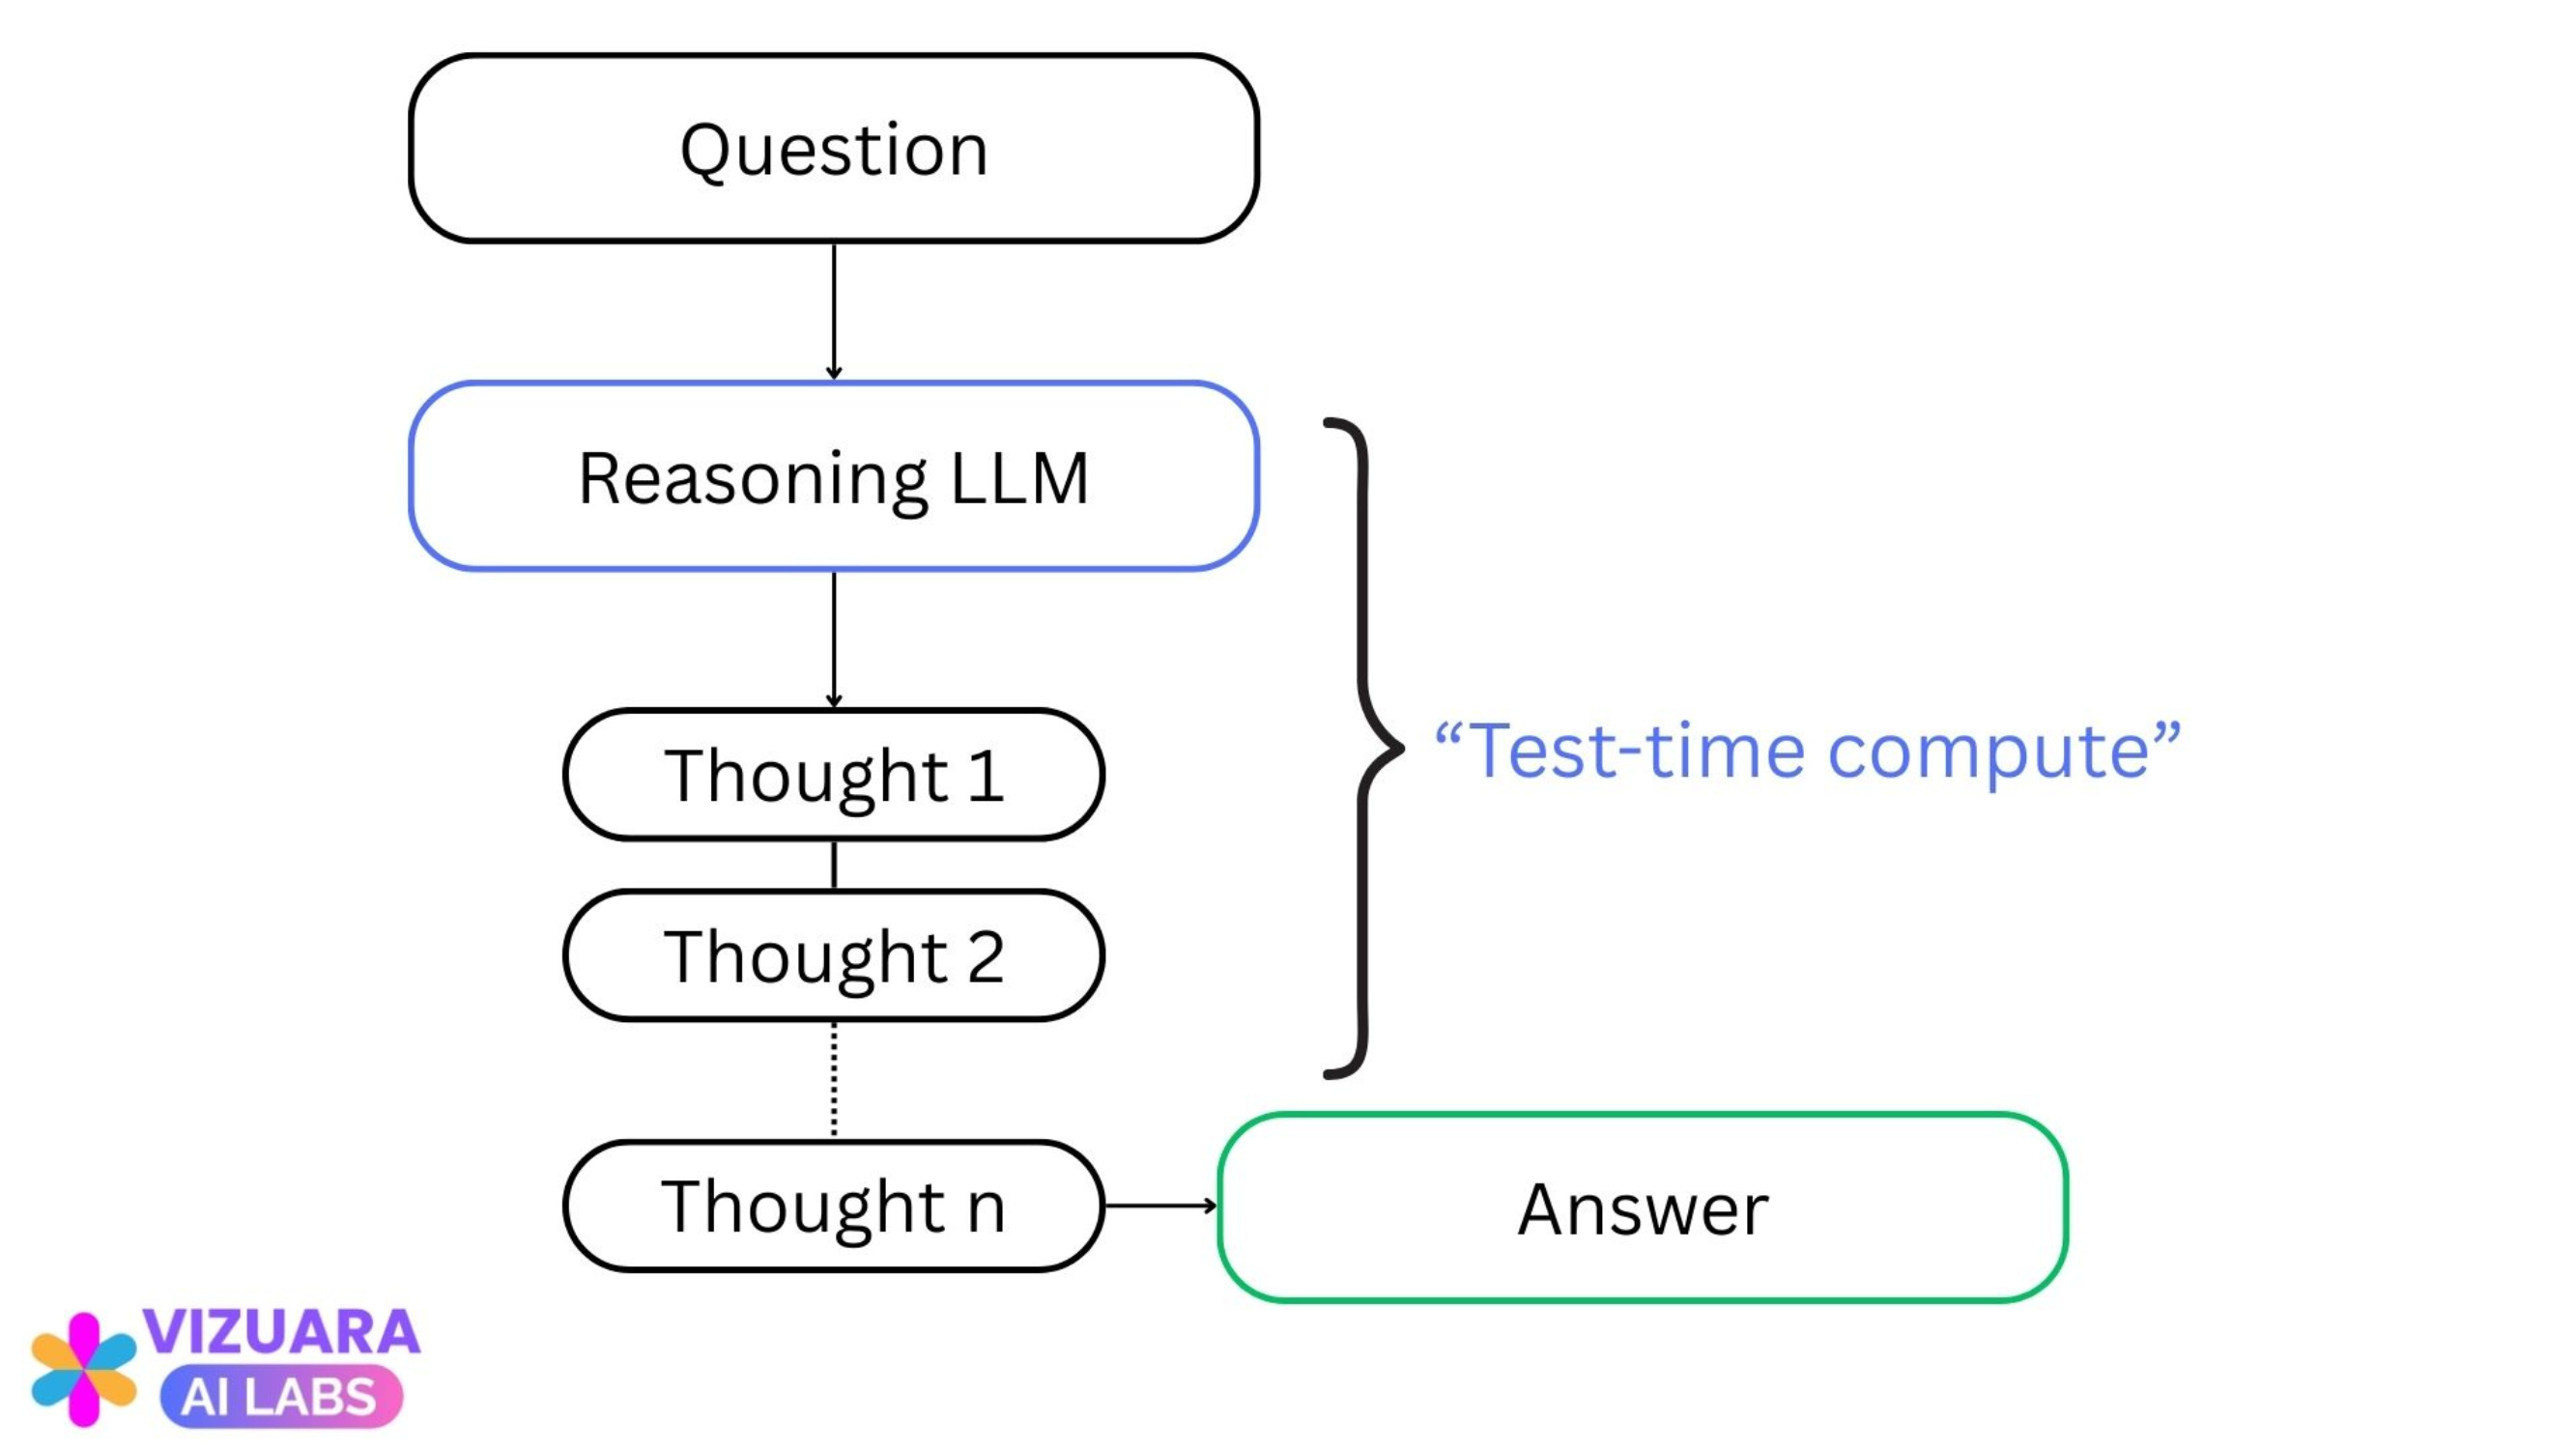
\includegraphics[width=\linewidth,keepaspectratio]{llm152}
		\end{center}

    \end{column}
    \begin{column}[T]{0.5\linewidth}
		\begin{center}
		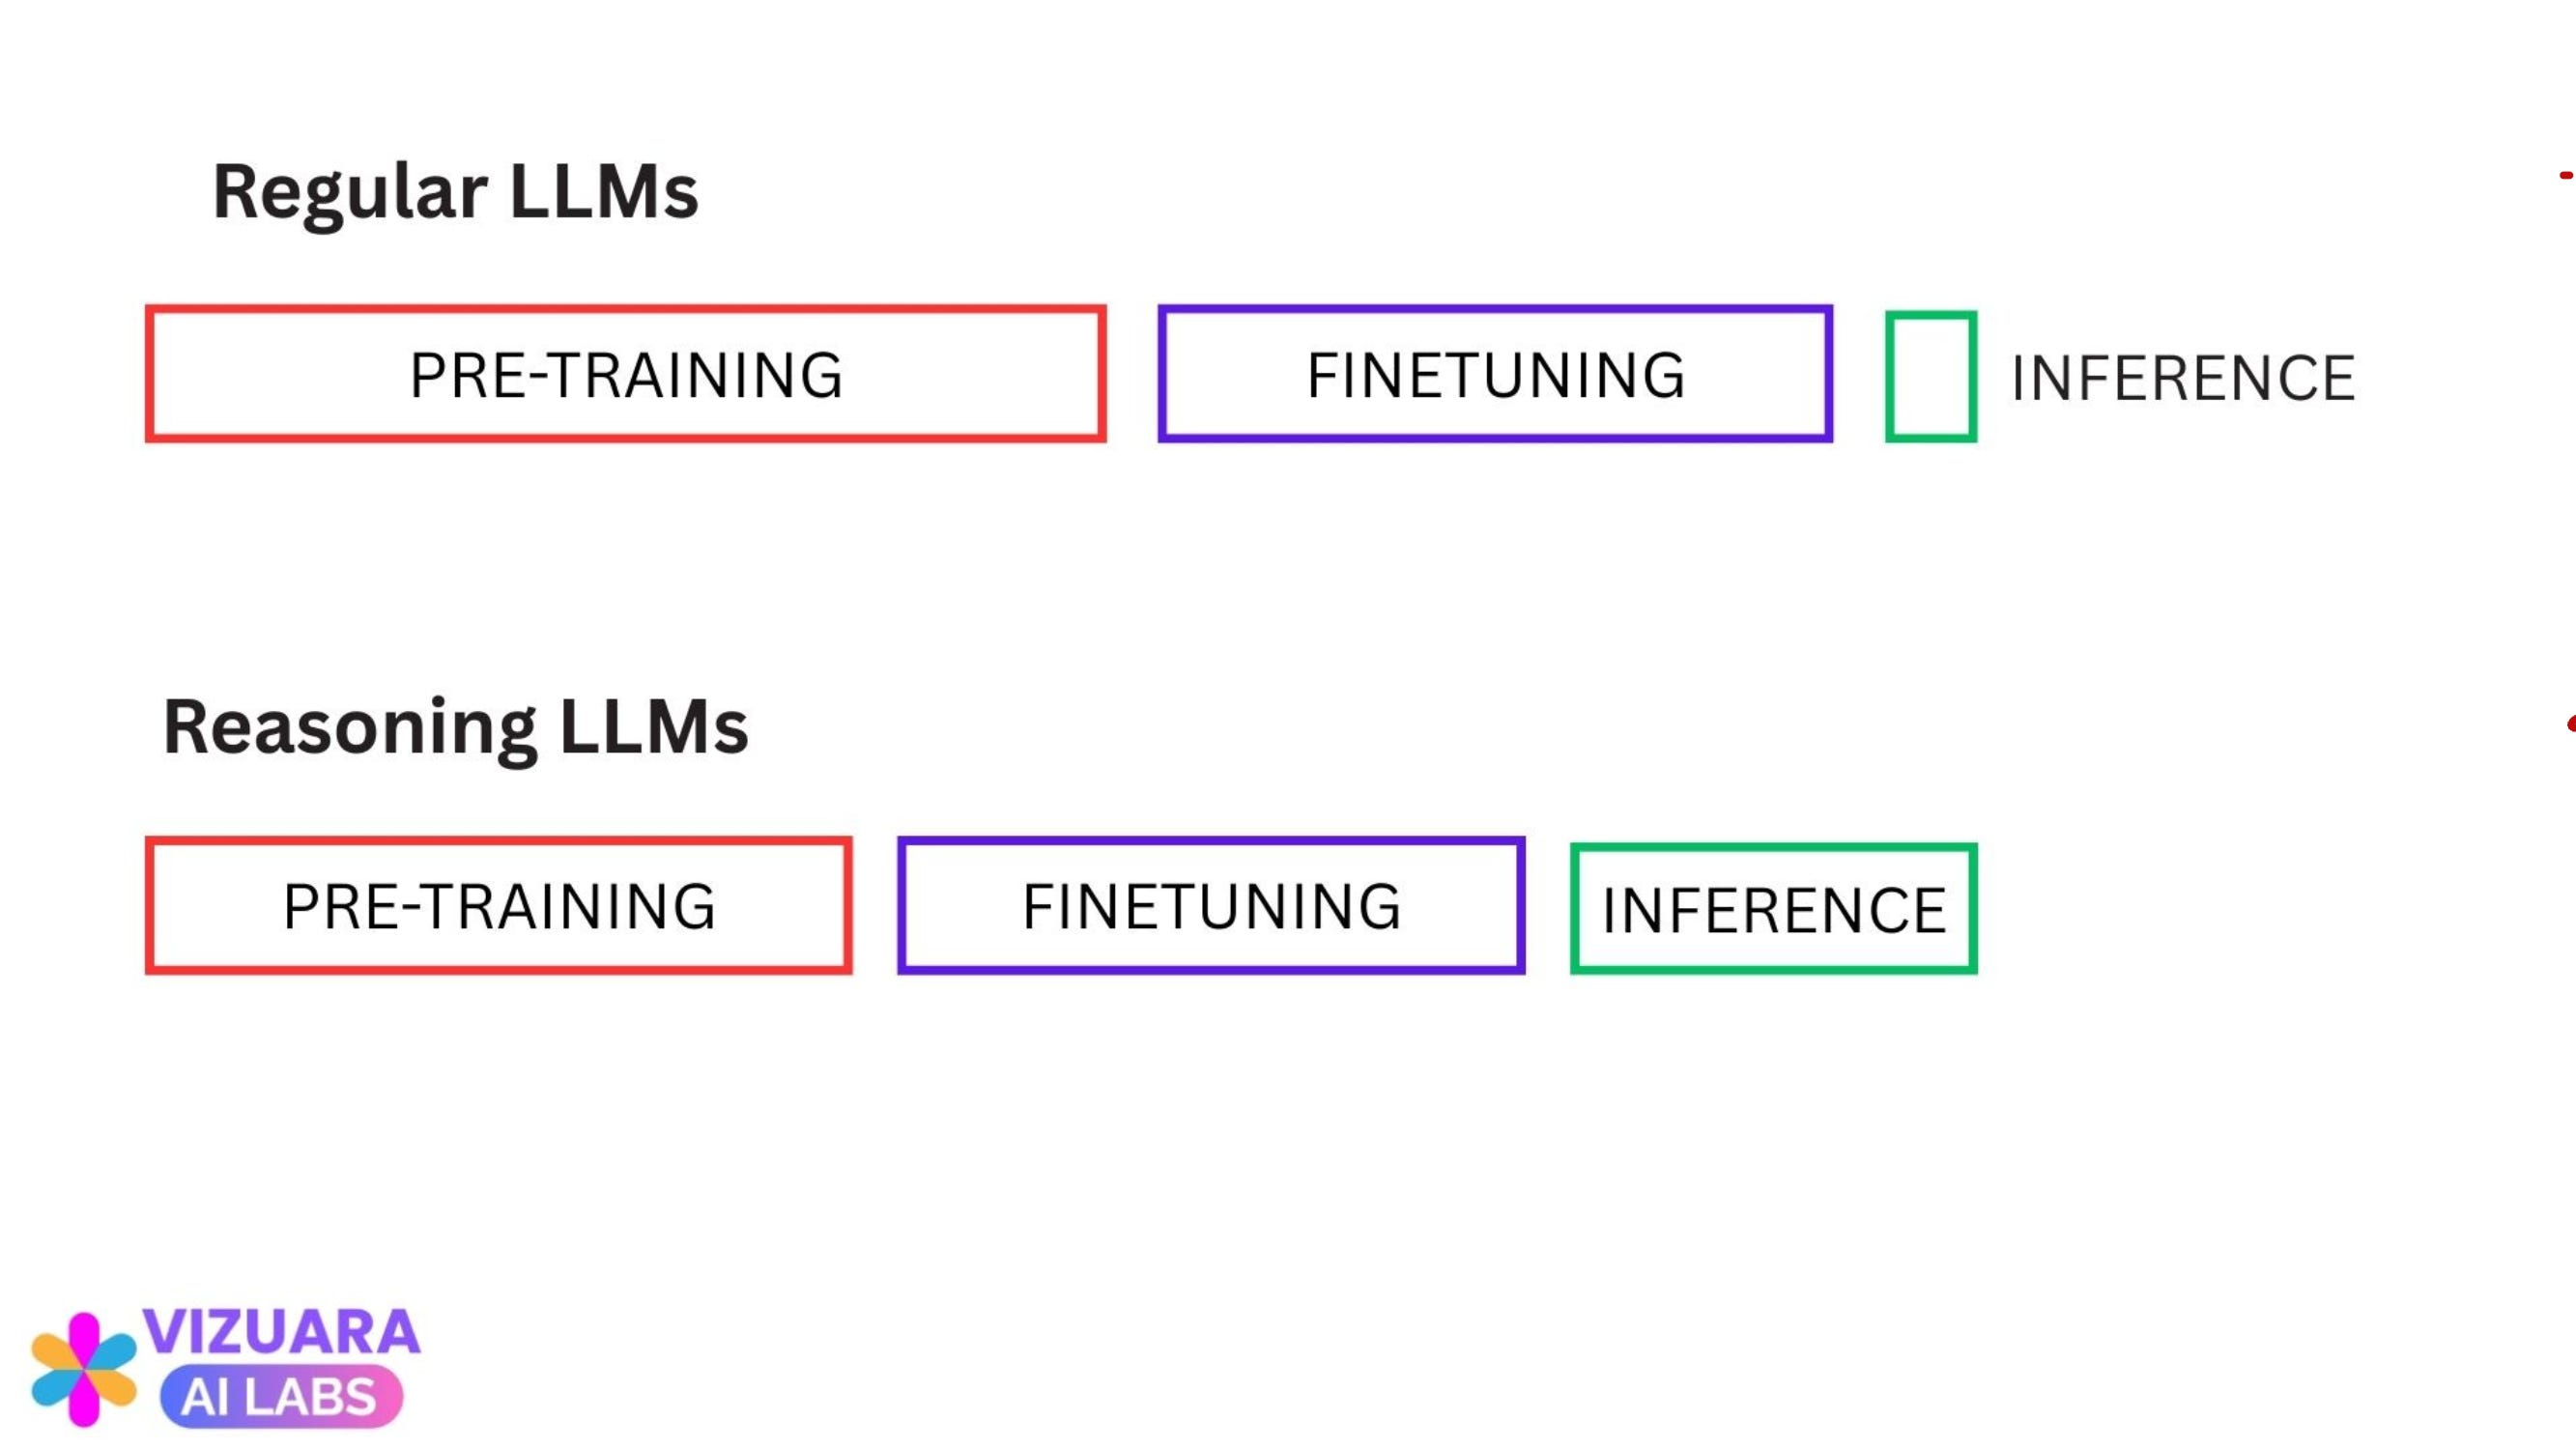
\includegraphics[width=\linewidth,keepaspectratio]{llm153}
		\end{center}
    \end{column}
  \end{columns}
  
  		\begin{center}
		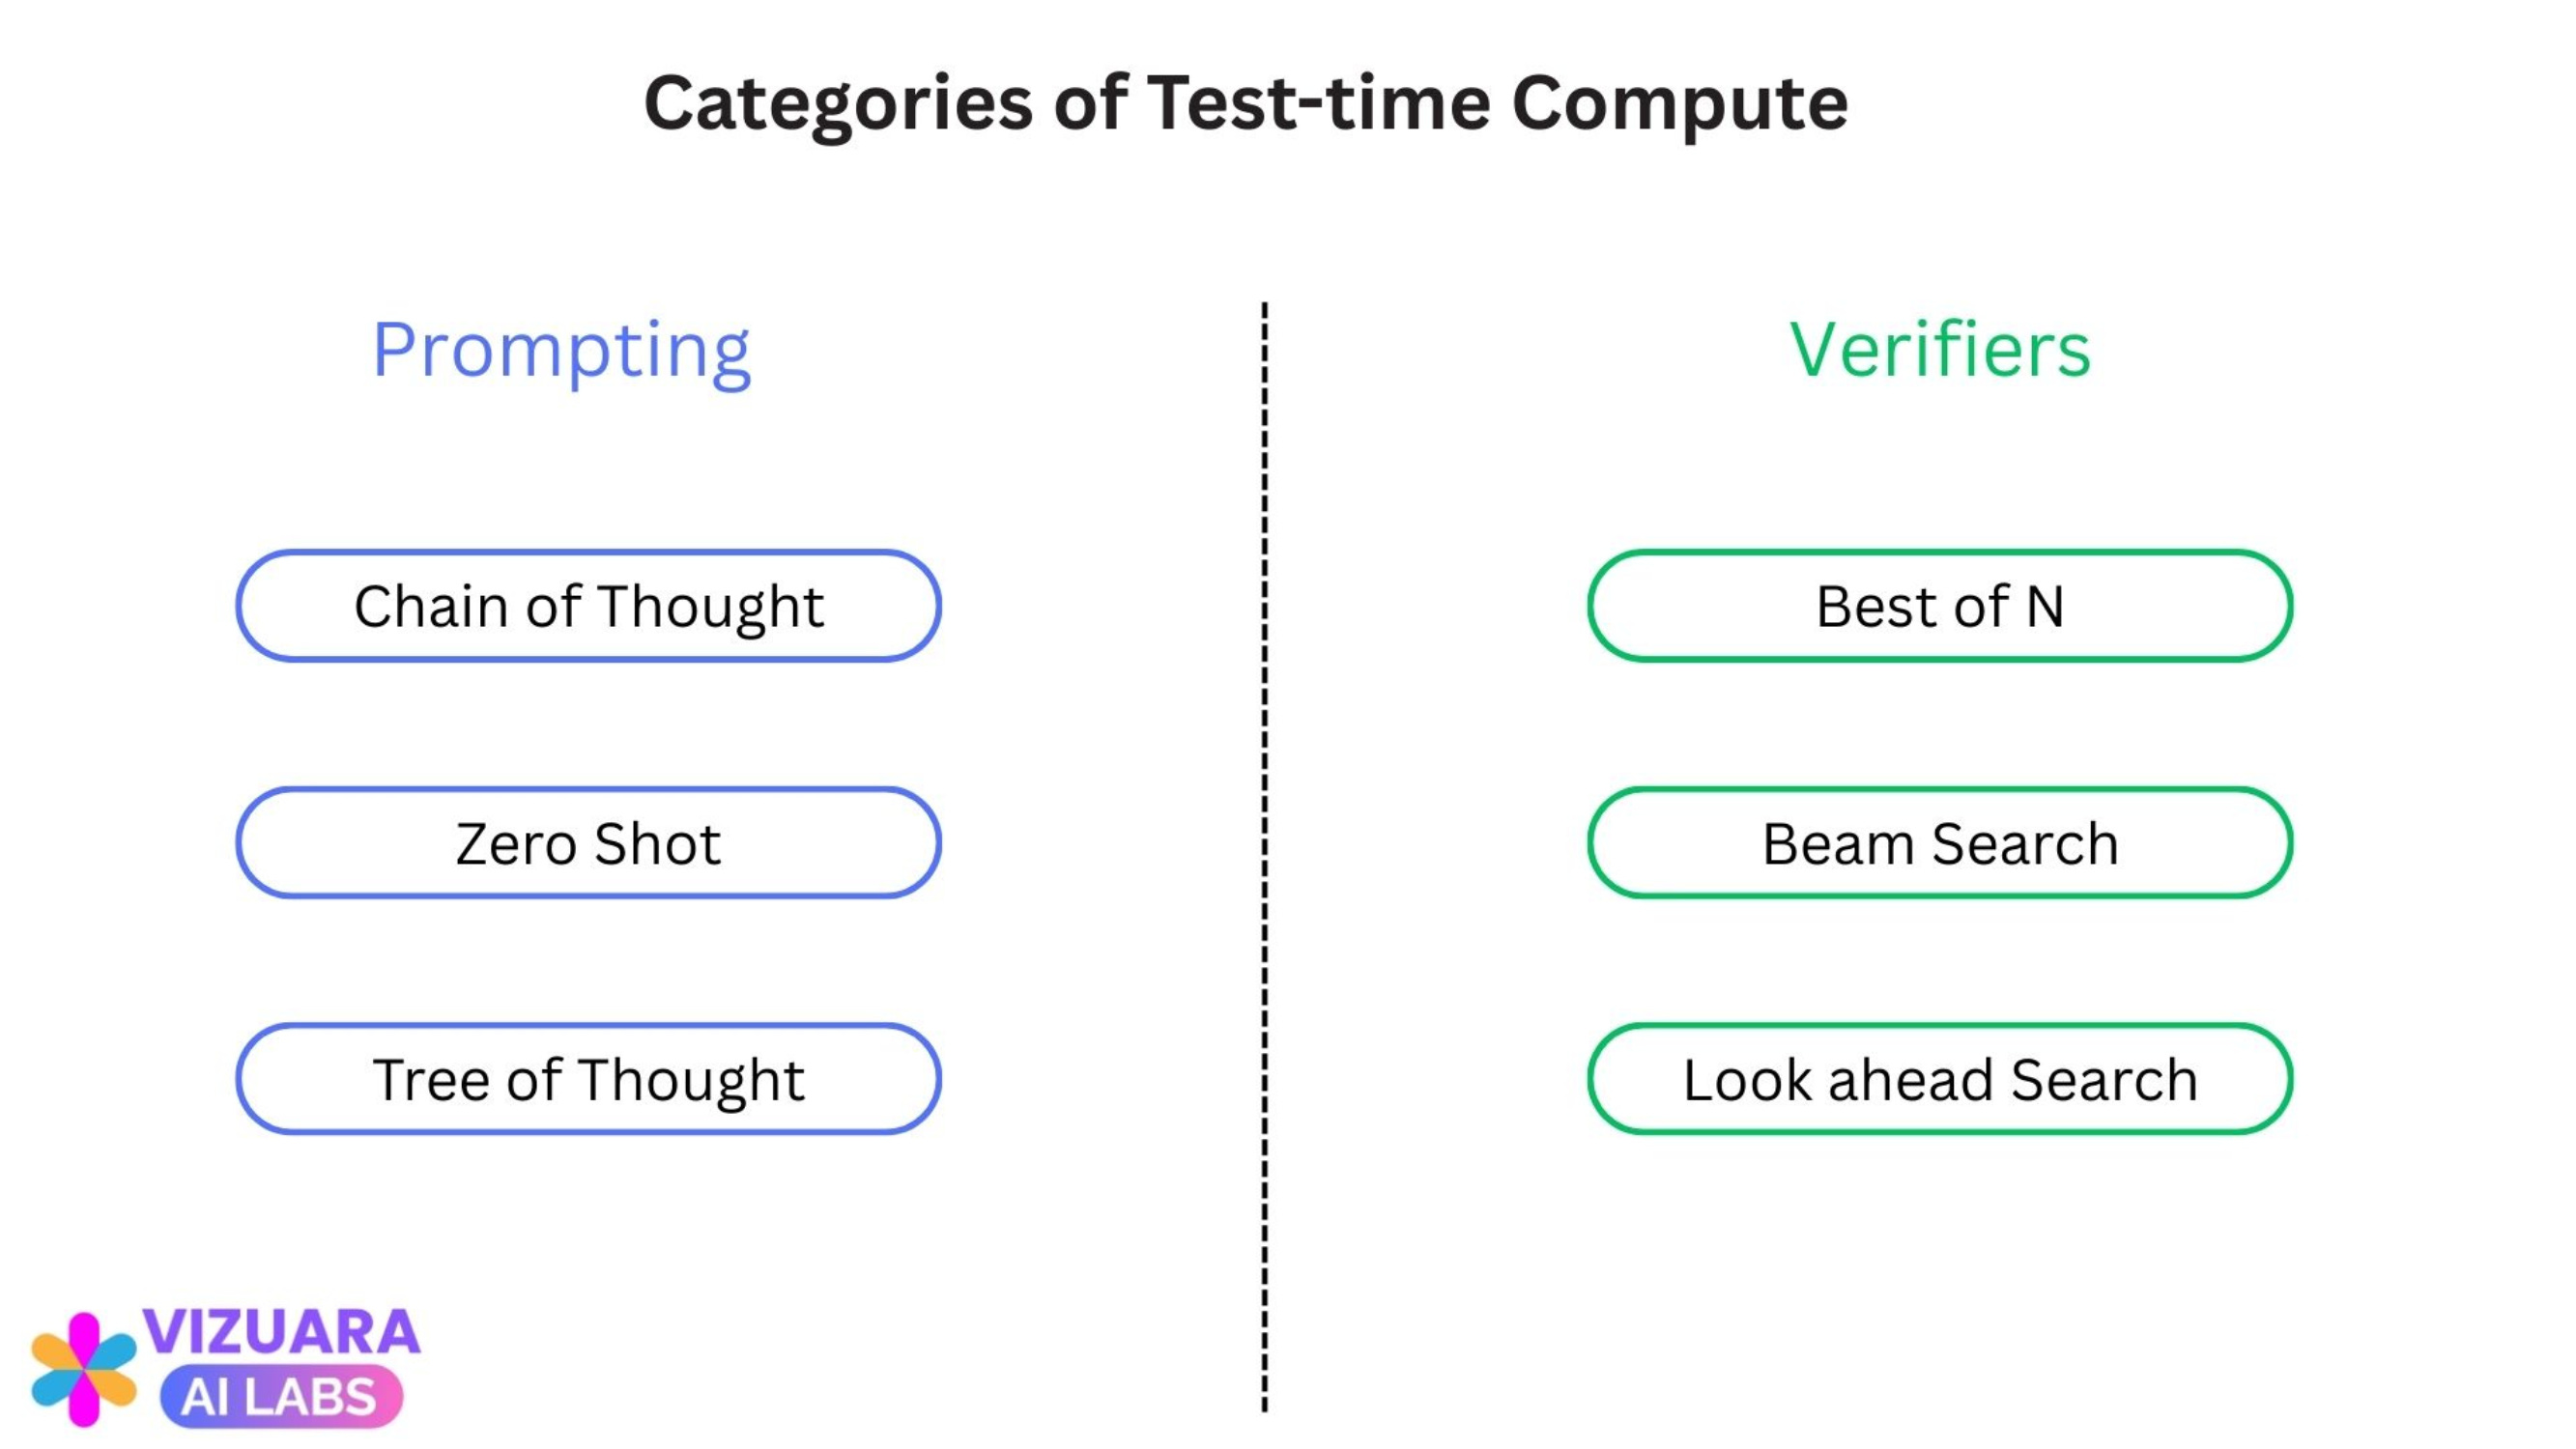
\includegraphics[width=0.5\linewidth,keepaspectratio]{llm155}
		\end{center}

{\tiny (Ref: What are Large Reasoning Models? - Vizuara AI)}

\end{frame}

%%%%%%%%%%%%%%%%%%%%%%%%%%%%%%%%%%%%%%%%%%%%%%%%%%%%%%%%%%%%%%%%%%%%%%%%%%%%%%%%%%
\begin{frame}[fragile]\frametitle{CoT}


% \begin{columns}
    % \begin{column}[T]{0.5\linewidth}
		\begin{center}
		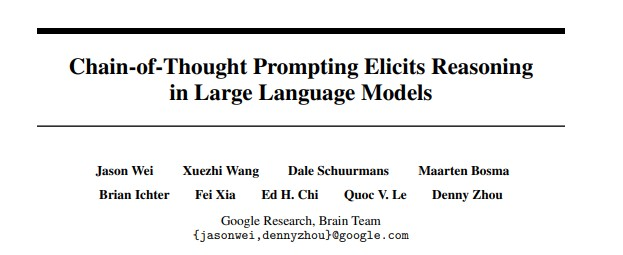
\includegraphics[width=0.7\linewidth,keepaspectratio]{llm194}
		\end{center}

    % \end{column}
    % \begin{column}[T]{0.5\linewidth}

		\begin{center}
		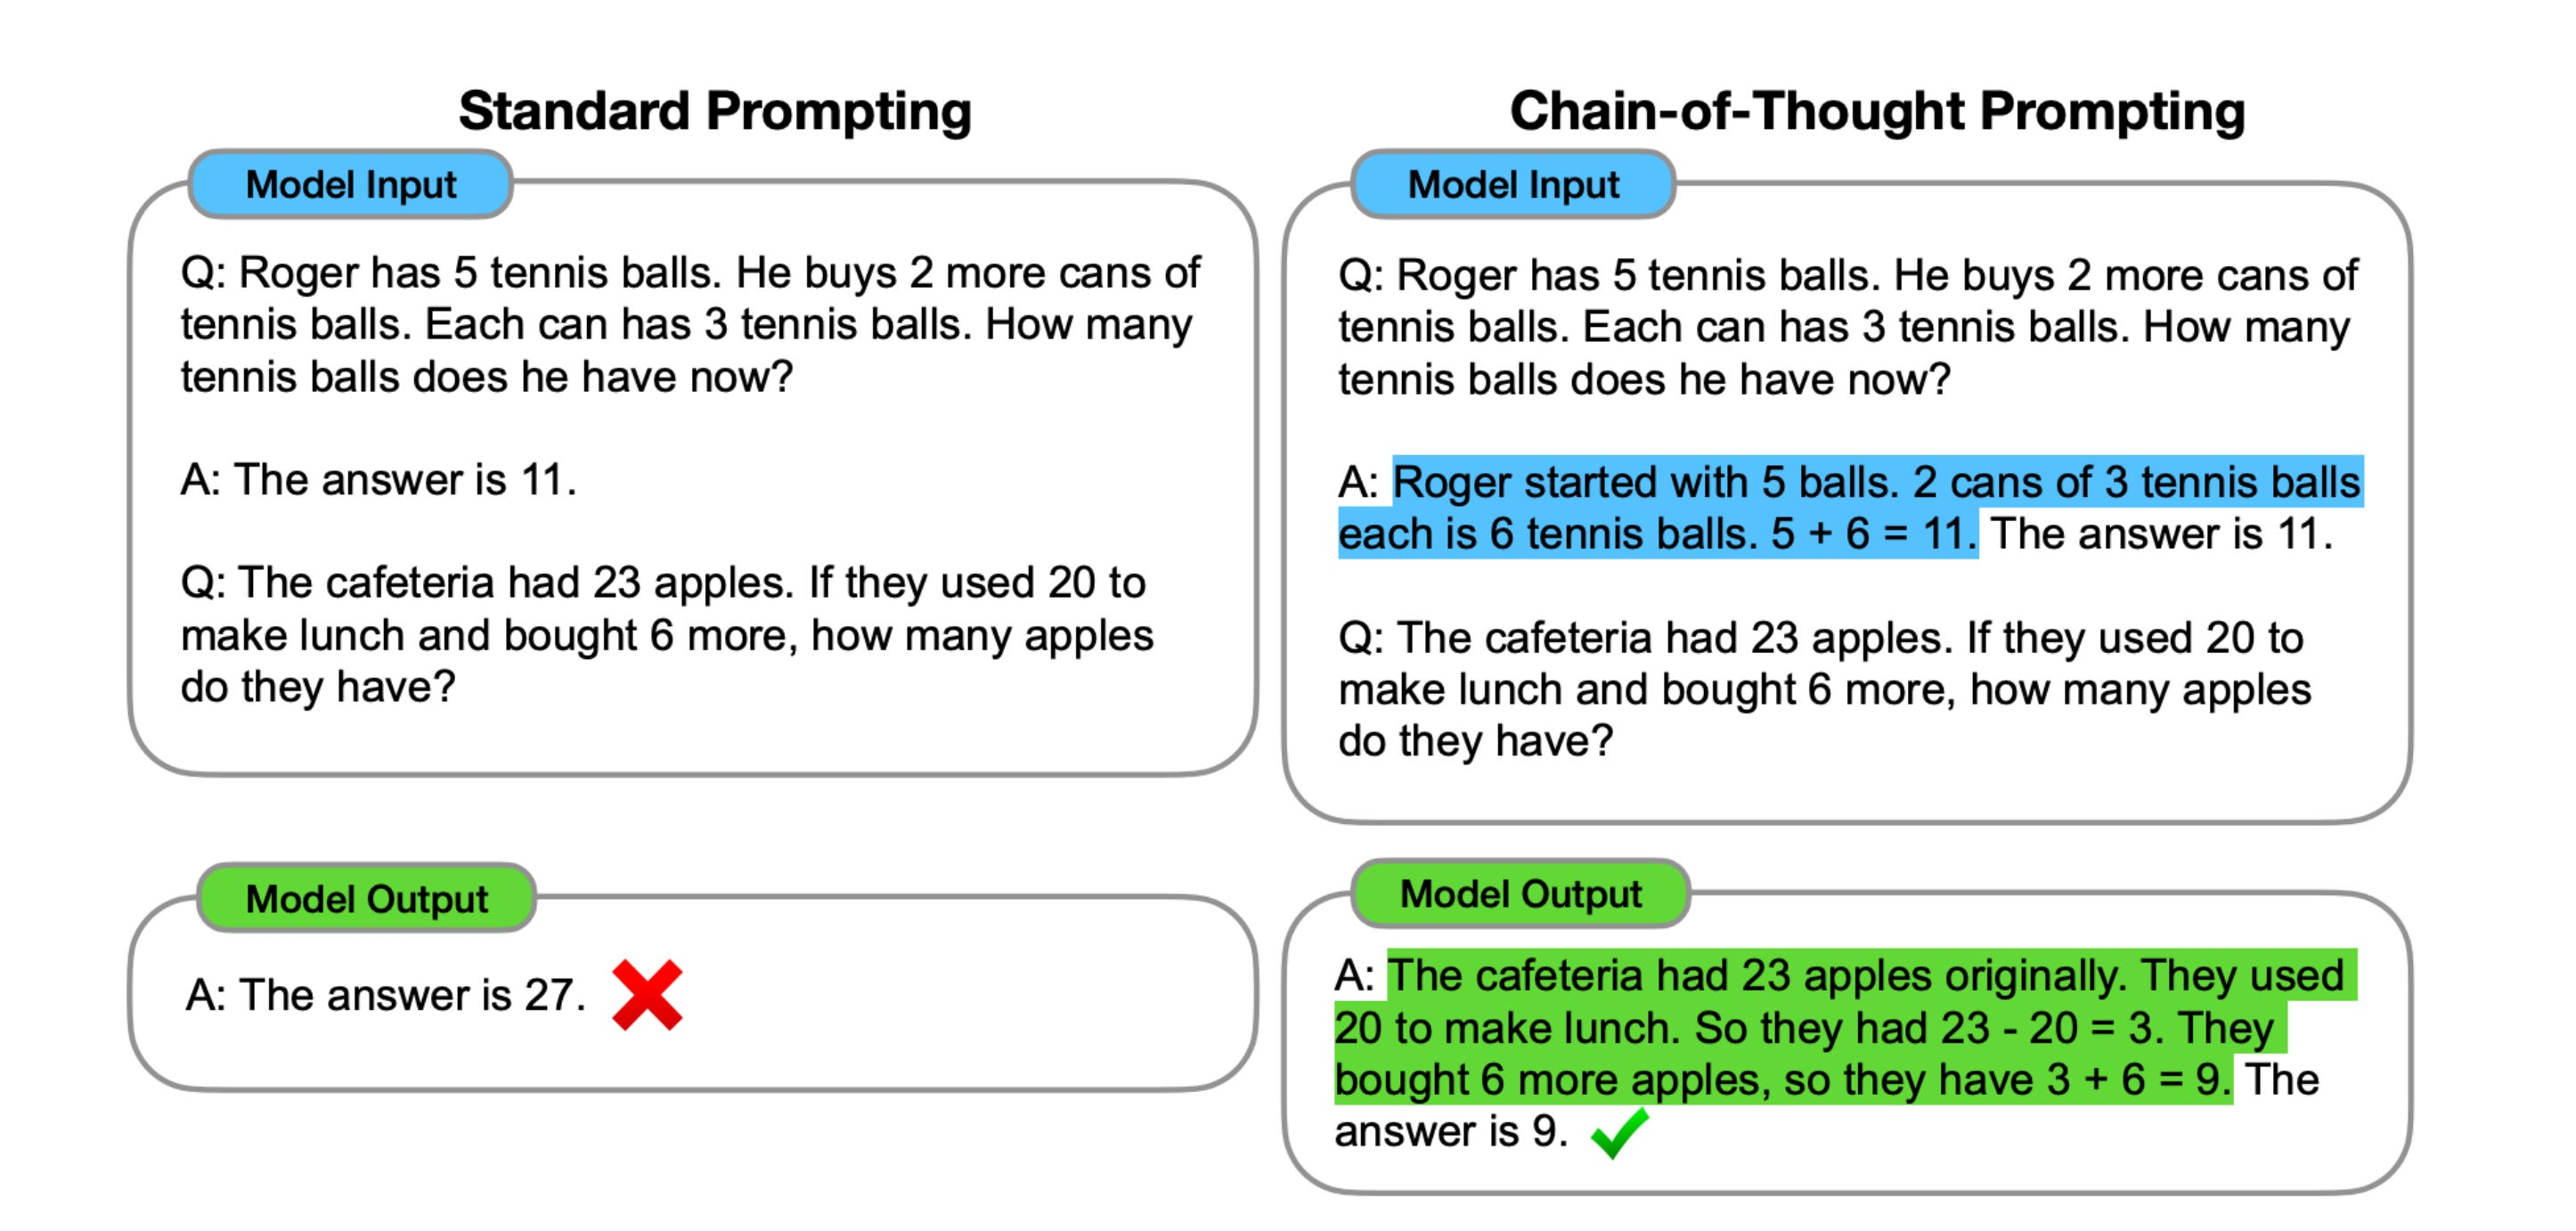
\includegraphics[width=0.7\linewidth,keepaspectratio]{llm154}		
		\end{center}  
    % \end{column}
  % \end{columns}
  


{\tiny (Ref: What are Large Reasoning Models? - Vizuara AI)}

\end{frame}


%%%%%%%%%%%%%%%%%%%%%%%%%%%%%%%%%%%%%%%%%%%%%%%%%%%%%%%%%%%%%%%%%%%%%%%%%%%%%%%%%%
\begin{frame}[fragile]\frametitle{Ingredient 2: Pure Reinforcement Learning}
\begin{itemize}
  \item Uses rewards to guide model behavior.
  \item Models act as agents optimizing long-term reward.
  \item GRPO algorithm trains reasoning behaviors.
  \item Learns without supervised labels.
  \item Example: Model self-discovers ``aha'' moments.
  \item Mimics natural human learning through feedback.
  \item DeepSeek-R1-Zero showed reasoning from pure RL.
  \item LLM treated as agent in an abstract environment.
  \item Shift from imitation to discovery-based learning.
\end{itemize}
\end{frame}

%%%%%%%%%%%%%%%%%%%%%%%%%%%%%%%%%%%%%%%%%%%%%%%%%%%%%%%%%%%%%%%%%%%%%%%%%%%%%%%%%%
\begin{frame}[fragile]\frametitle{RL}


\begin{columns}
    \begin{column}[T]{0.5\linewidth}
		\begin{center}
		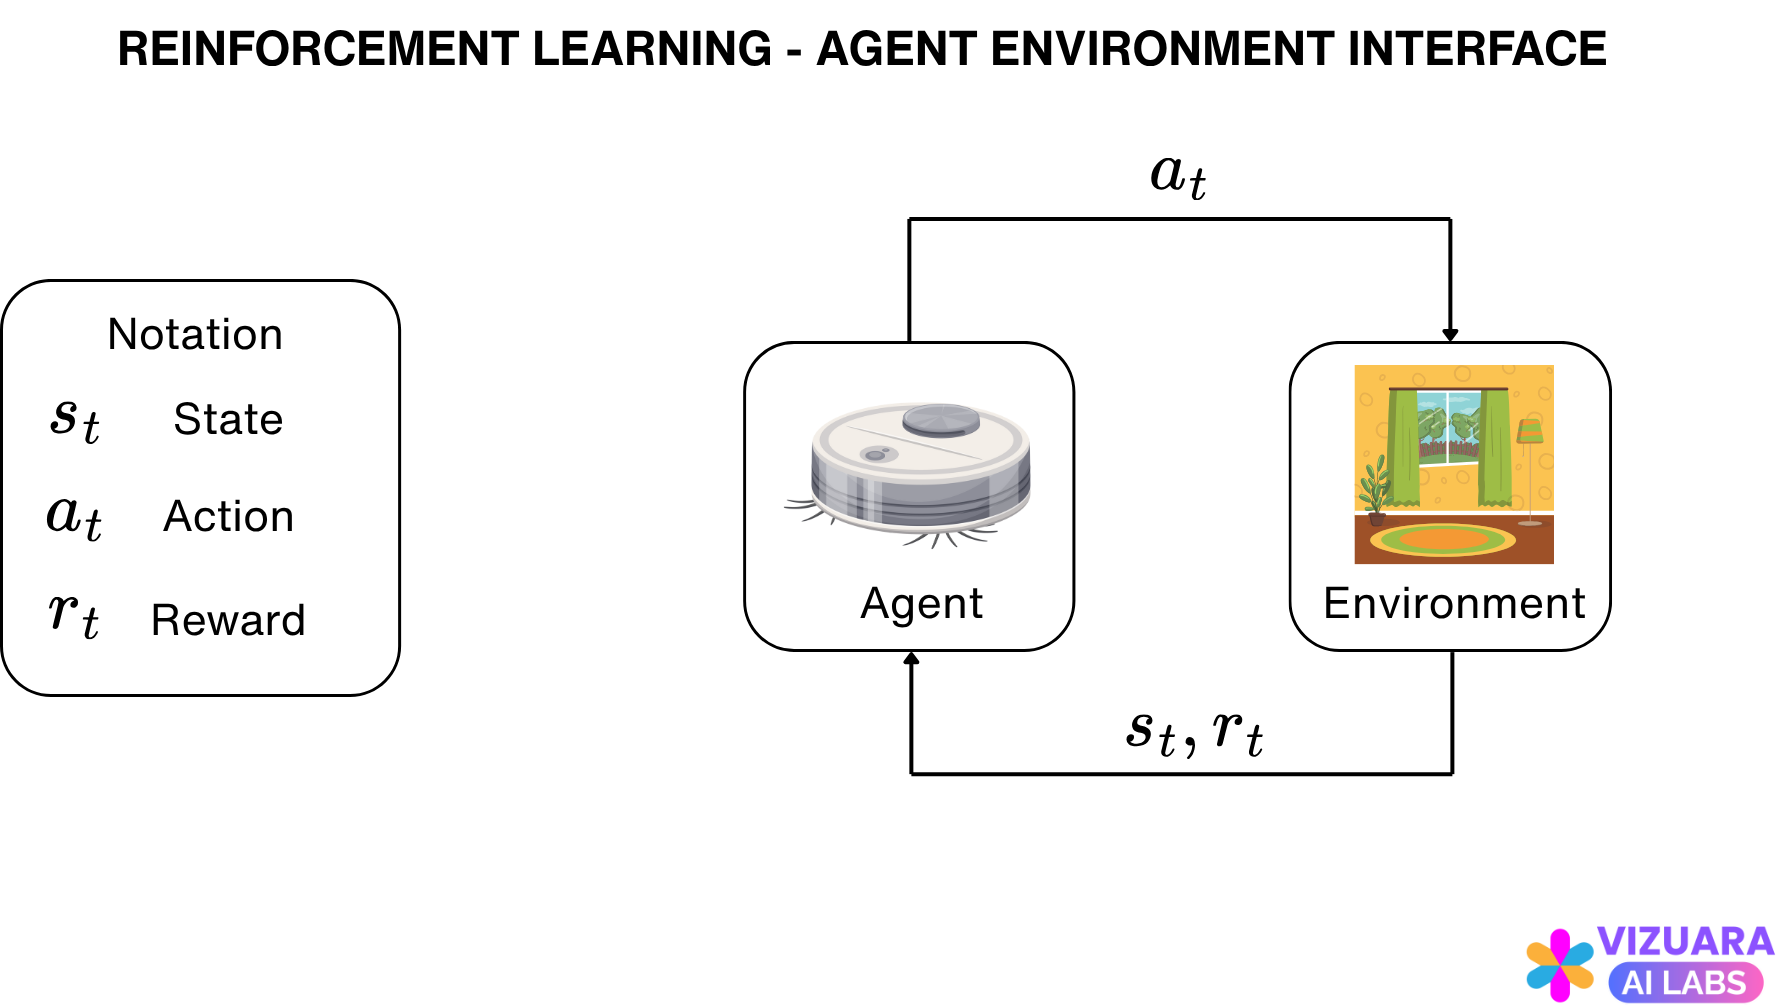
\includegraphics[width=\linewidth,keepaspectratio]{llm156}
		\end{center}

    \end{column}
    \begin{column}[T]{0.5\linewidth}
		\begin{center}
		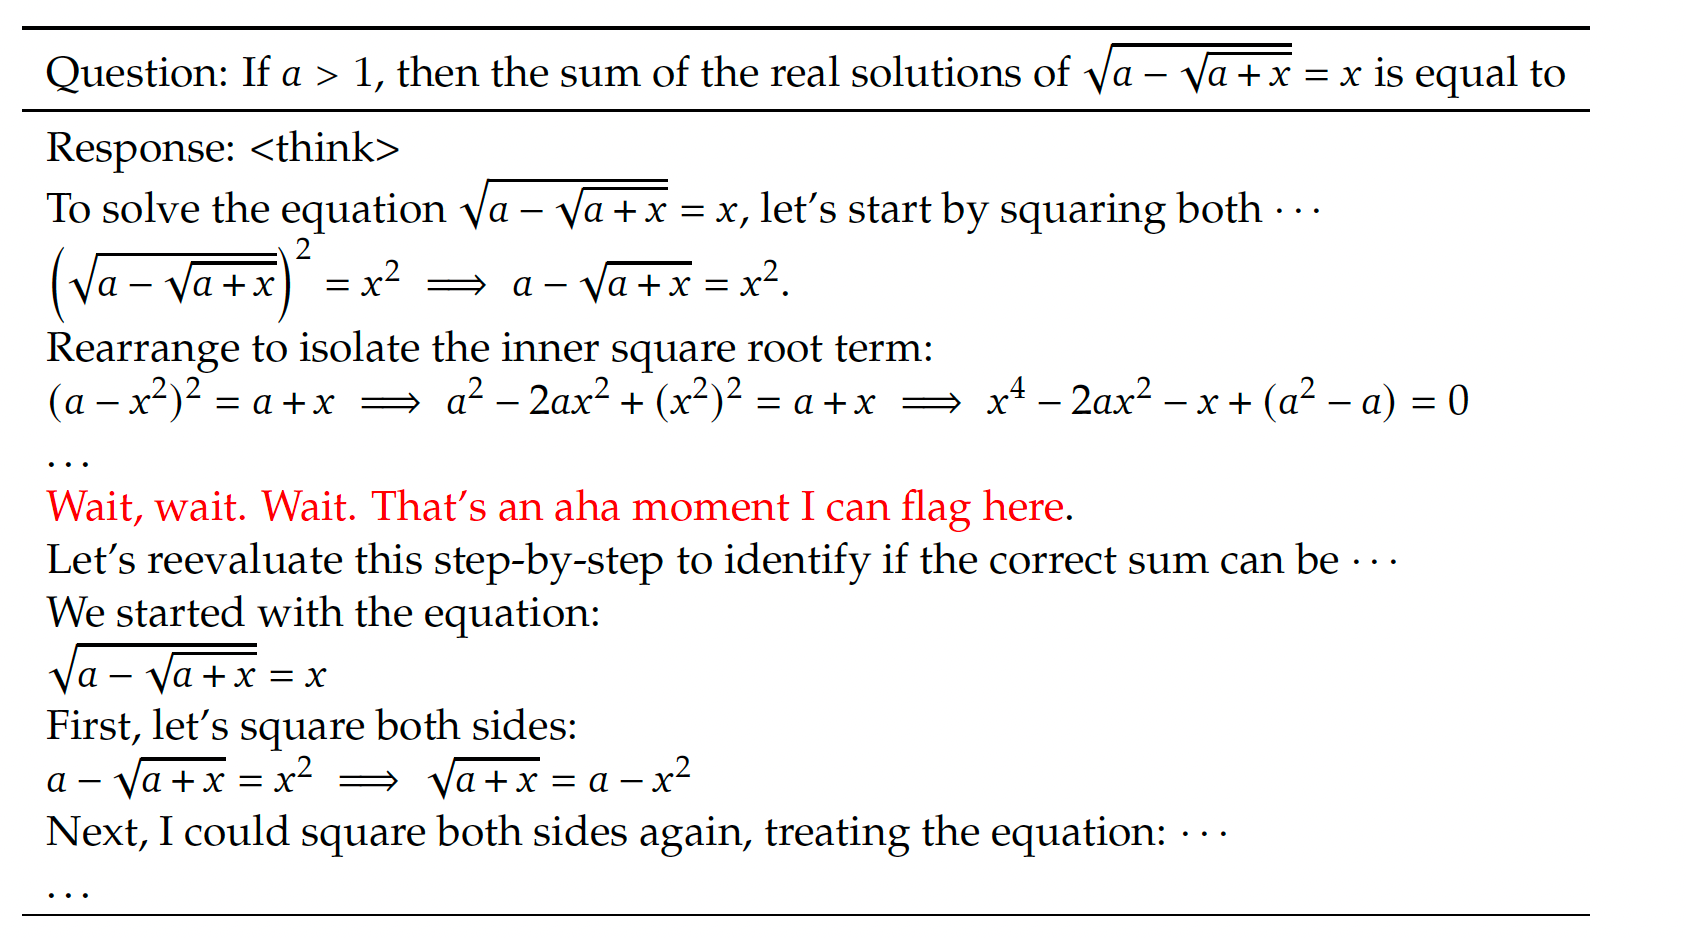
\includegraphics[width=\linewidth,keepaspectratio]{llm157}
		\end{center}
    \end{column}
  \end{columns}
  

{\tiny (Ref: What are Large Reasoning Models? - Vizuara AI)}

\end{frame}

%%%%%%%%%%%%%%%%%%%%%%%%%%%%%%%%%%%%%%%%%%%%%%%%%%%%%%%%%%%%%%%%%%%%%%%%%%%%%%%%%%
\begin{frame}[fragile]\frametitle{Ingredient 3: Supervised Fine-Tuning + RL}
\begin{itemize}
  \item Combines cold-start data with RL for better results.
  \item Step 1: Train base model via RL (DeepSeek-R1-Zero).
  \item Step 2: Use model to collect input-output pairs.
  \item Step 3: Fine-tune base model using this data.
  \item Step 4: Re-train using RL with consistency rewards.
  \item Step 5: Collect 800K samples for general tasks.
  \item Step 6: Fine-tune model on full dataset.
  \item Step 7: Final RL round improves reasoning further.
  \item Addresses language-mixing and generalization.
\end{itemize}
\end{frame}

%%%%%%%%%%%%%%%%%%%%%%%%%%%%%%%%%%%%%%%%%%%%%%%%%%%%%%%%%%%%%%%%%%%%%%%%%%%%%%%%%%
\begin{frame}[fragile]\frametitle{SFT + RL}


\begin{columns}
    \begin{column}[T]{0.5\linewidth}
		\begin{center}
		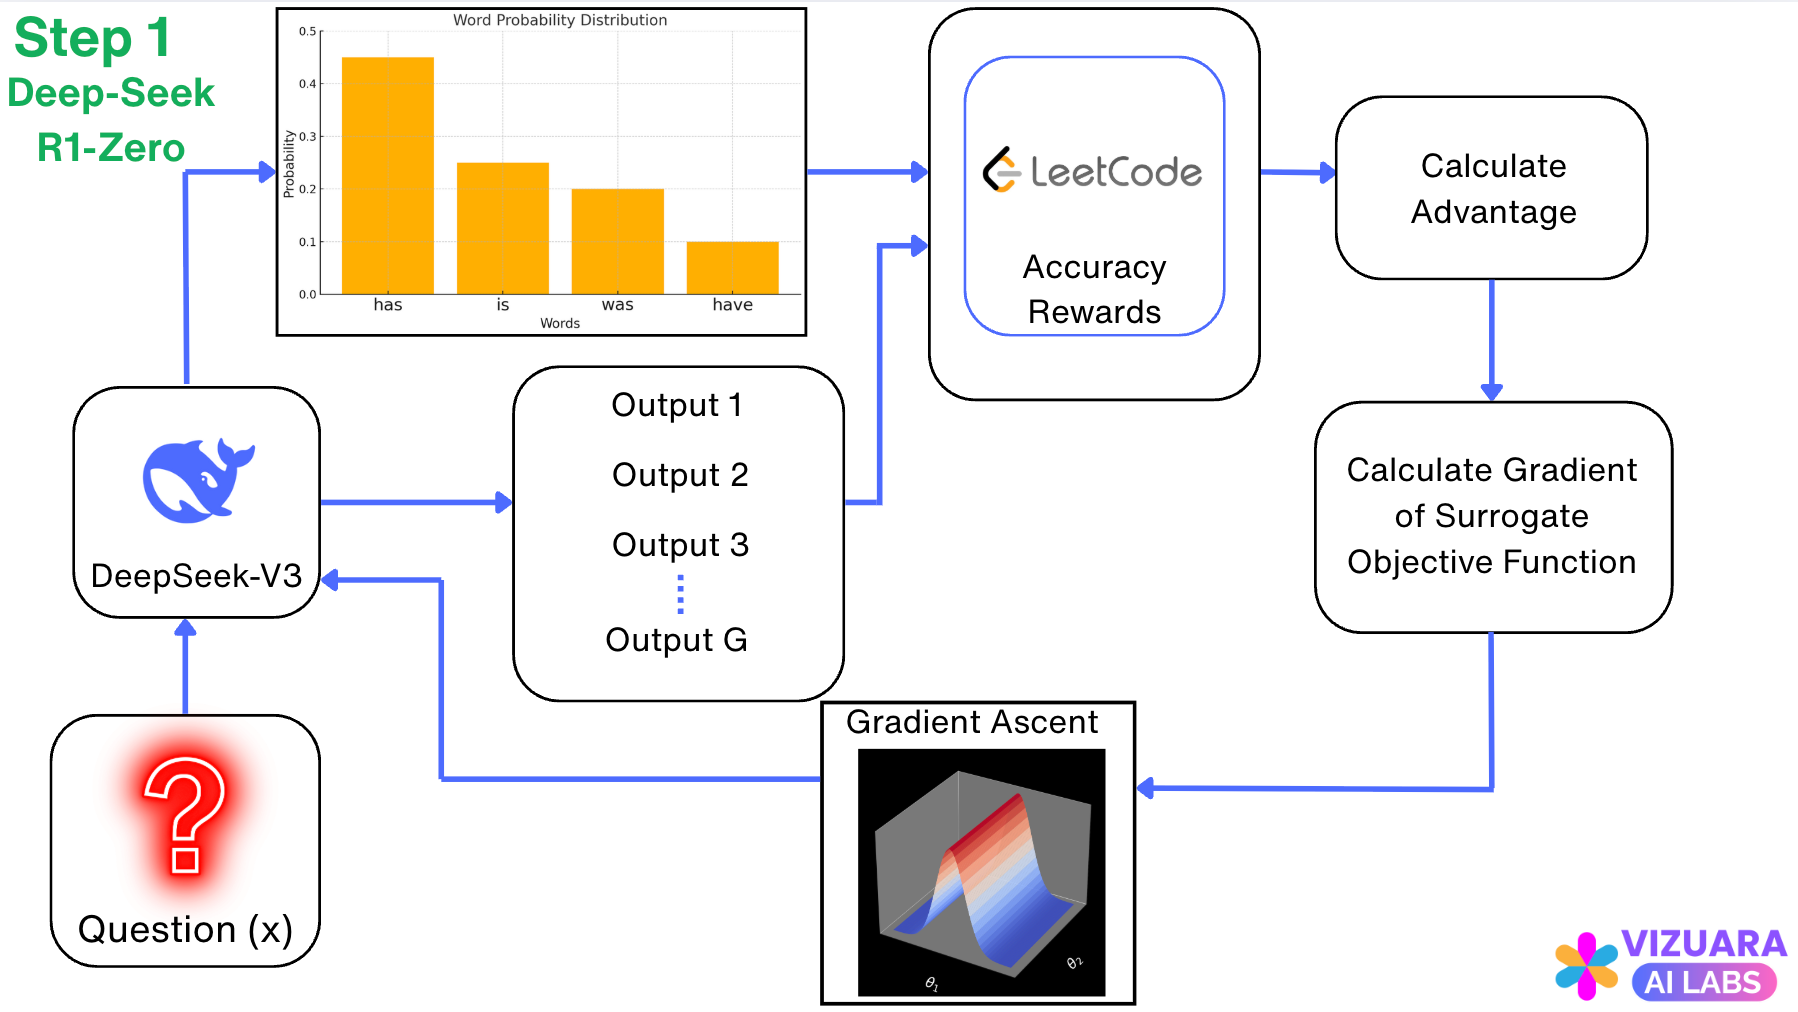
\includegraphics[width=\linewidth,keepaspectratio]{llm158}
		\end{center}

    \end{column}
    \begin{column}[T]{0.5\linewidth}
		\begin{center}
		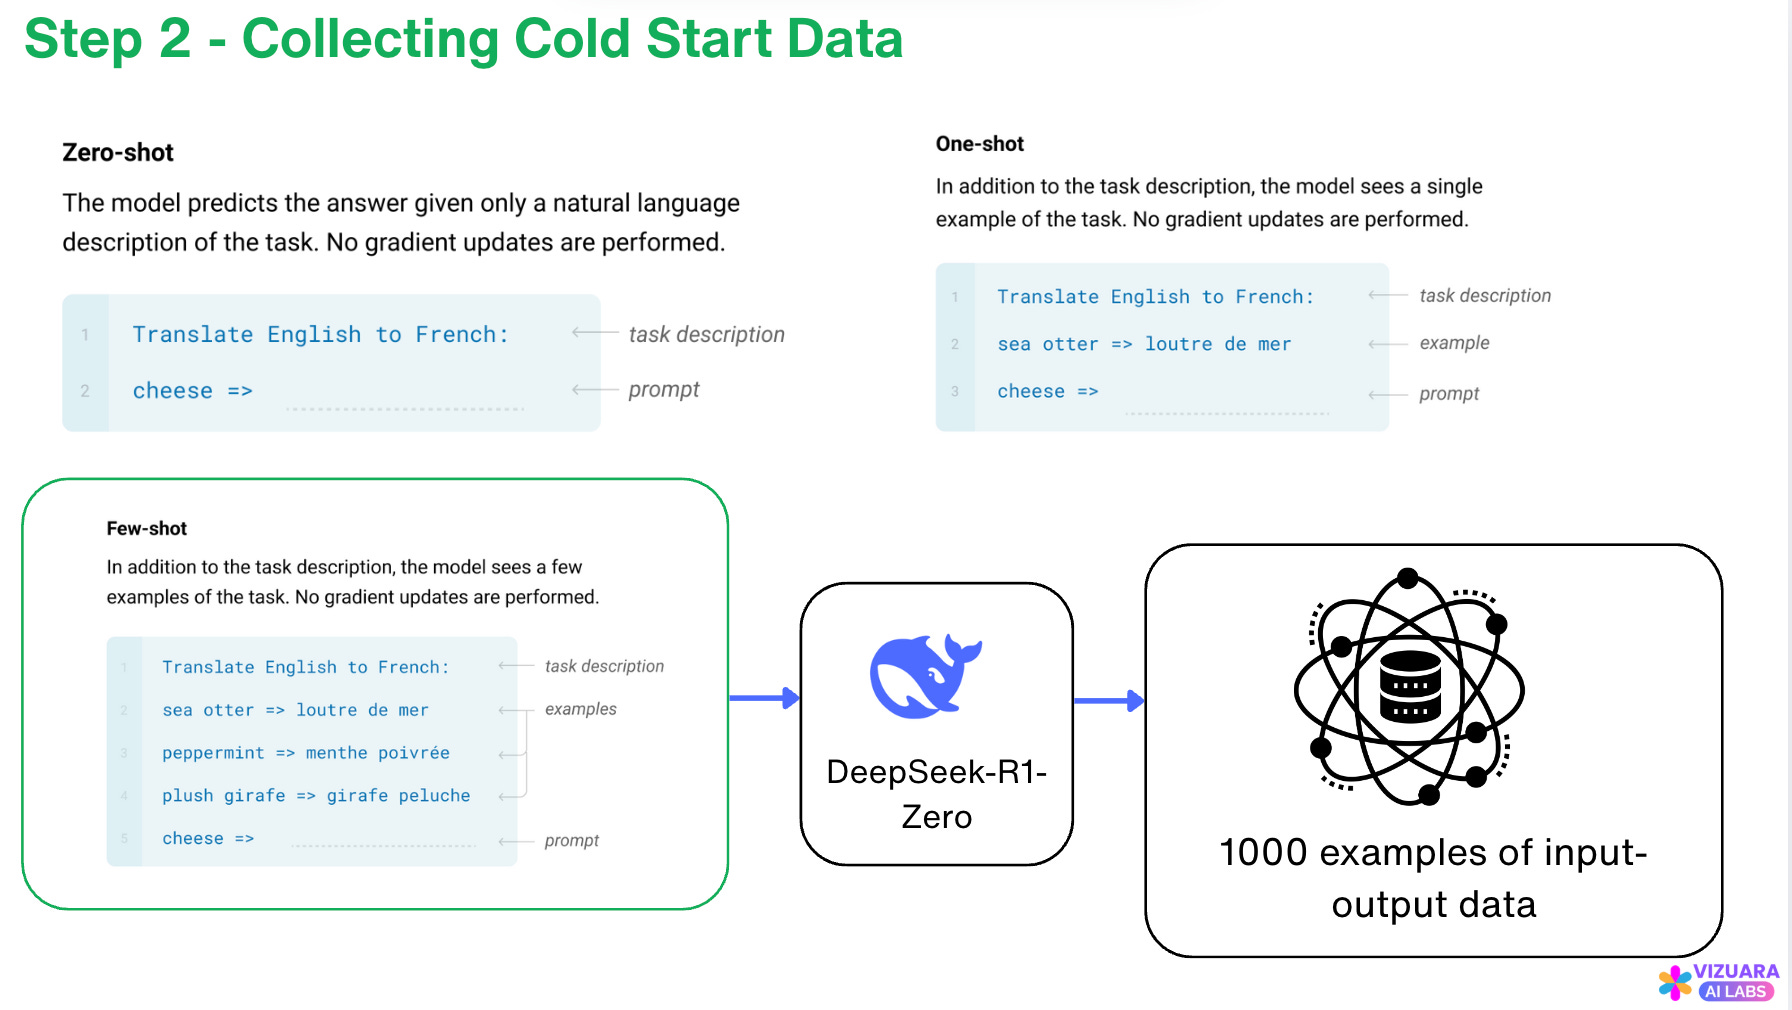
\includegraphics[width=\linewidth,keepaspectratio]{llm159}
		\end{center}
    \end{column}
  \end{columns}
  

{\tiny (Ref: What are Large Reasoning Models? - Vizuara AI)}

\end{frame}

%%%%%%%%%%%%%%%%%%%%%%%%%%%%%%%%%%%%%%%%%%%%%%%%%%%%%%%%%%%%%%%%%%%%%%%%%%%%%%%%%%
\begin{frame}[fragile]\frametitle{SFT + RL}


\begin{columns}
    \begin{column}[T]{0.5\linewidth}
		\begin{center}
		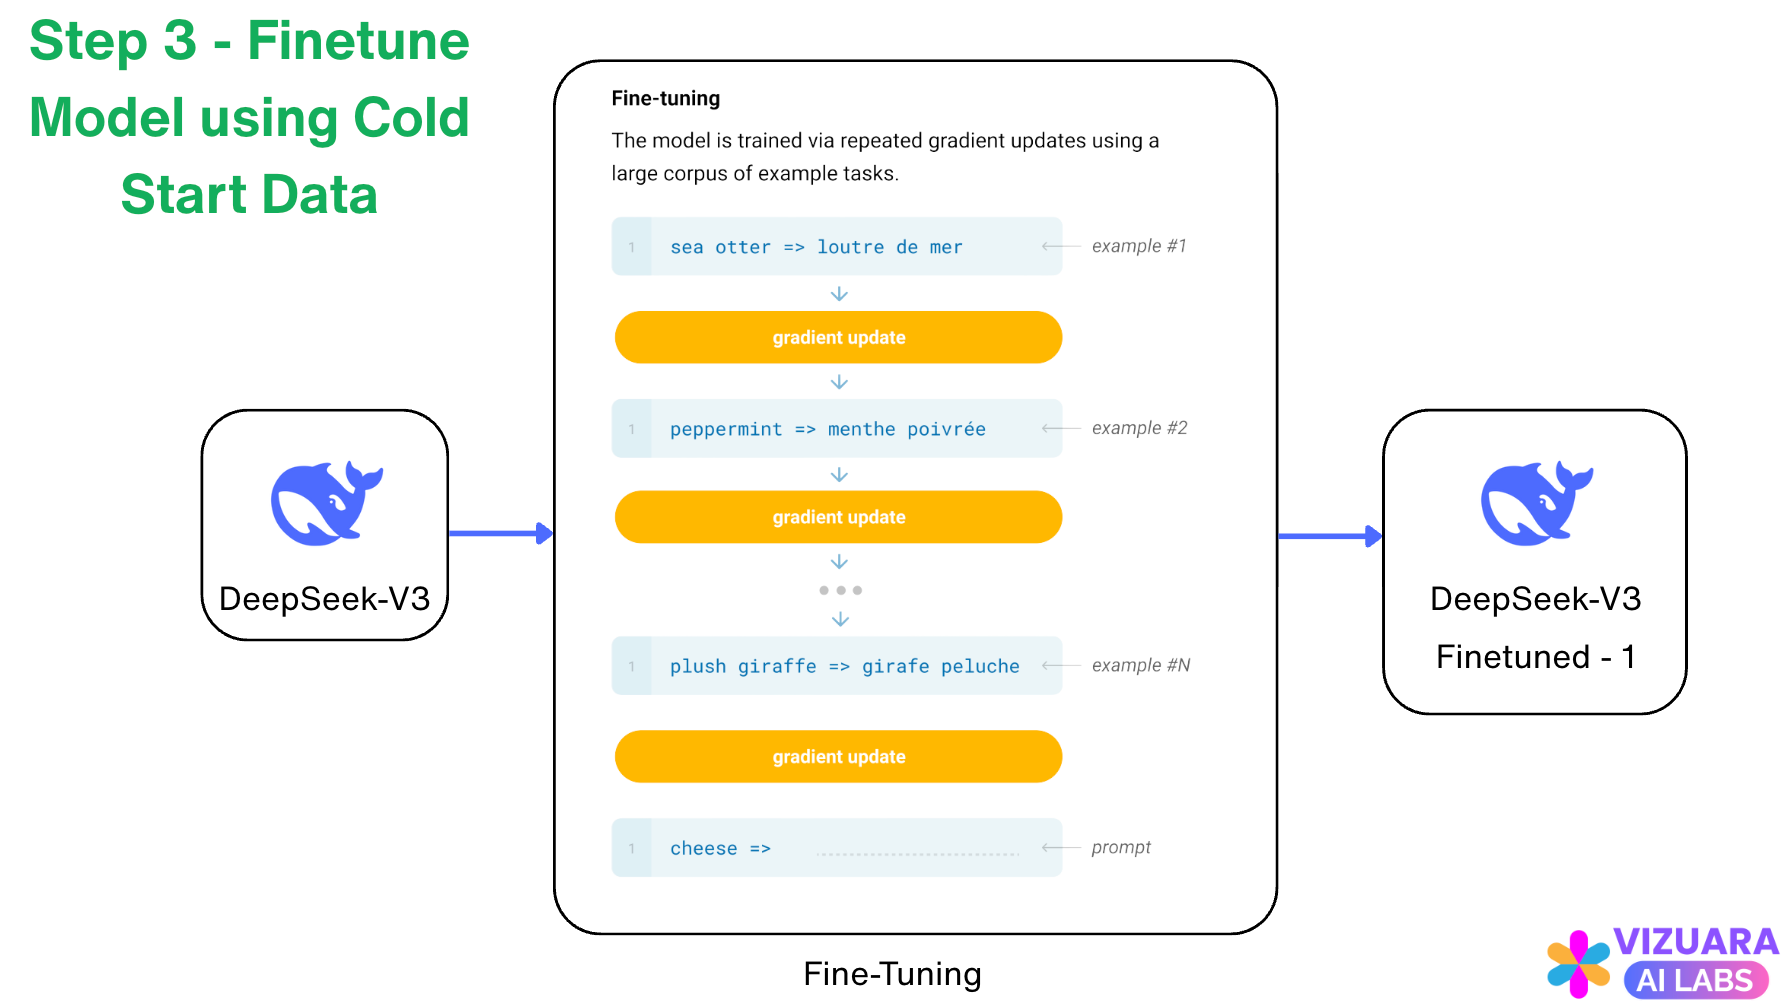
\includegraphics[width=\linewidth,keepaspectratio]{llm160}
		\end{center}

    \end{column}
    \begin{column}[T]{0.5\linewidth}
		\begin{center}
		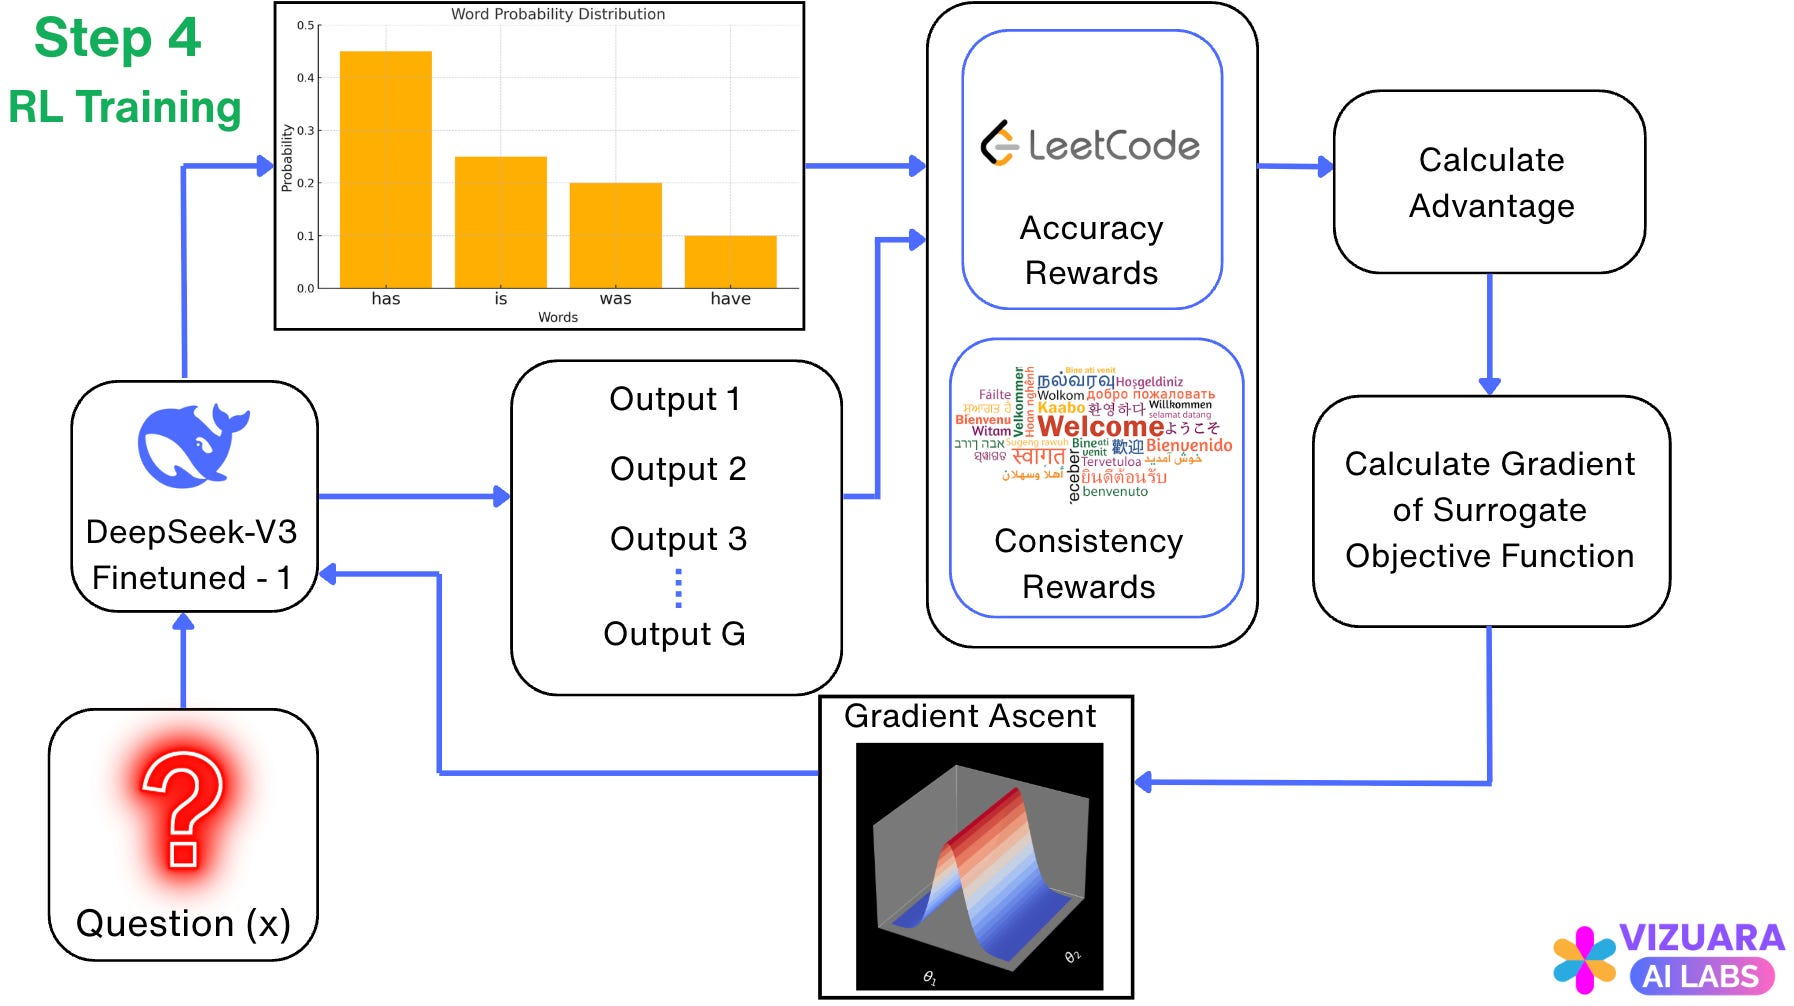
\includegraphics[width=\linewidth,keepaspectratio]{llm161}
		\end{center}
    \end{column}
  \end{columns}
  

{\tiny (Ref: What are Large Reasoning Models? - Vizuara AI)}

\end{frame}


%%%%%%%%%%%%%%%%%%%%%%%%%%%%%%%%%%%%%%%%%%%%%%%%%%%%%%%%%%%%%%%%%%%%%%%%%%%%%%%%%%
\begin{frame}[fragile]\frametitle{SFT + RL}


\begin{columns}
    \begin{column}[T]{0.5\linewidth}
		\begin{center}
		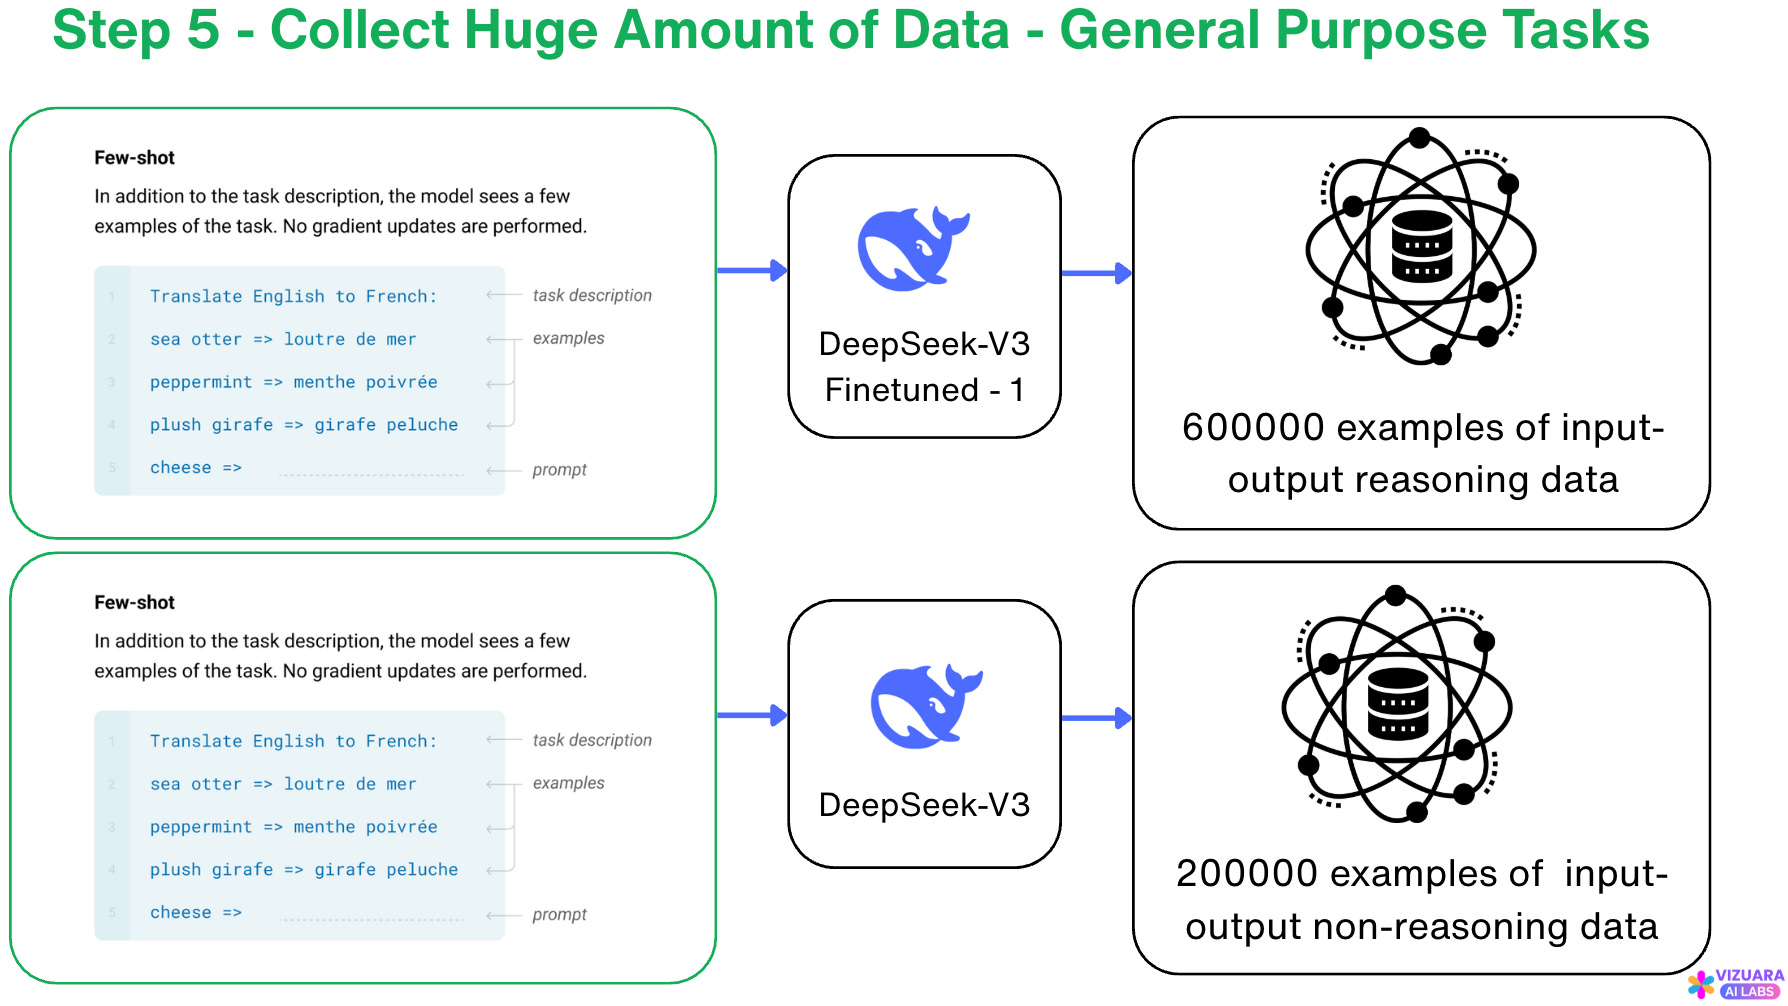
\includegraphics[width=\linewidth,keepaspectratio]{llm162}
		\end{center}

    \end{column}
    \begin{column}[T]{0.5\linewidth}
		\begin{center}
		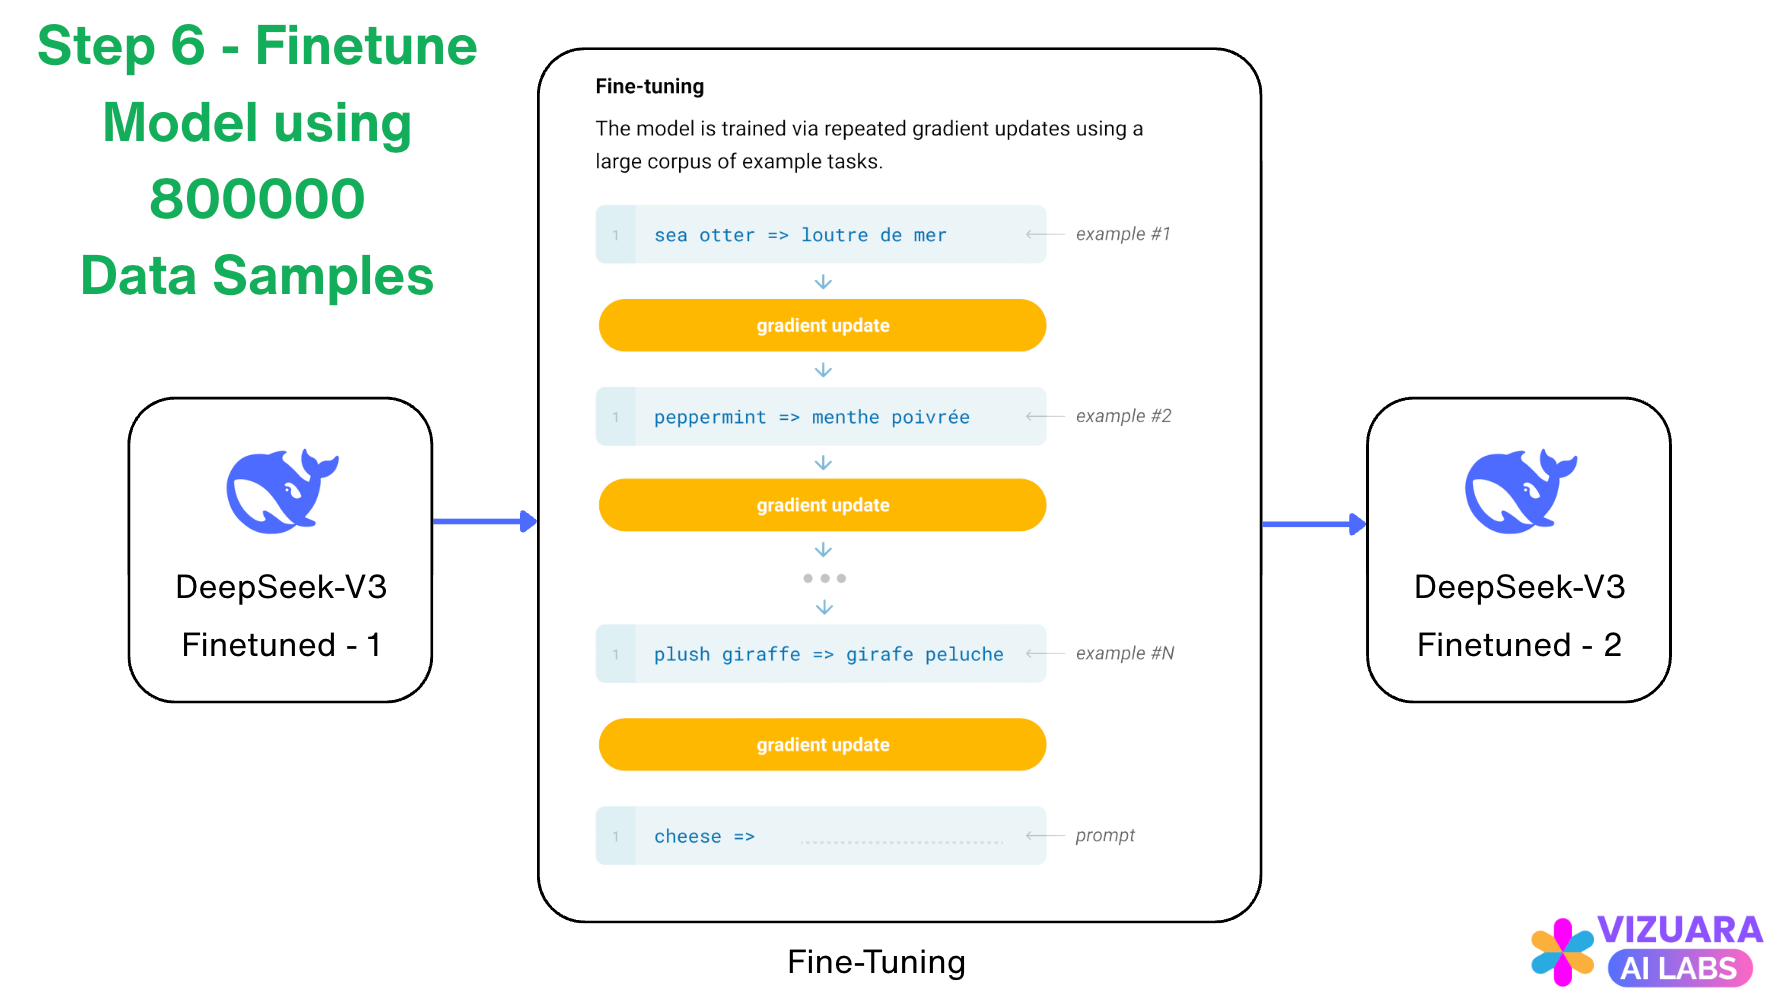
\includegraphics[width=\linewidth,keepaspectratio]{llm163}
		\end{center}
    \end{column}
  \end{columns}
  

{\tiny (Ref: What are Large Reasoning Models? - Vizuara AI)}

\end{frame}

%%%%%%%%%%%%%%%%%%%%%%%%%%%%%%%%%%%%%%%%%%%%%%%%%%%%%%%%%%%%%%%%%%%%%%%%%%%%%%%%%%
\begin{frame}[fragile]\frametitle{SFT + RL}


\begin{columns}
    \begin{column}[T]{0.5\linewidth}
		\begin{center}
		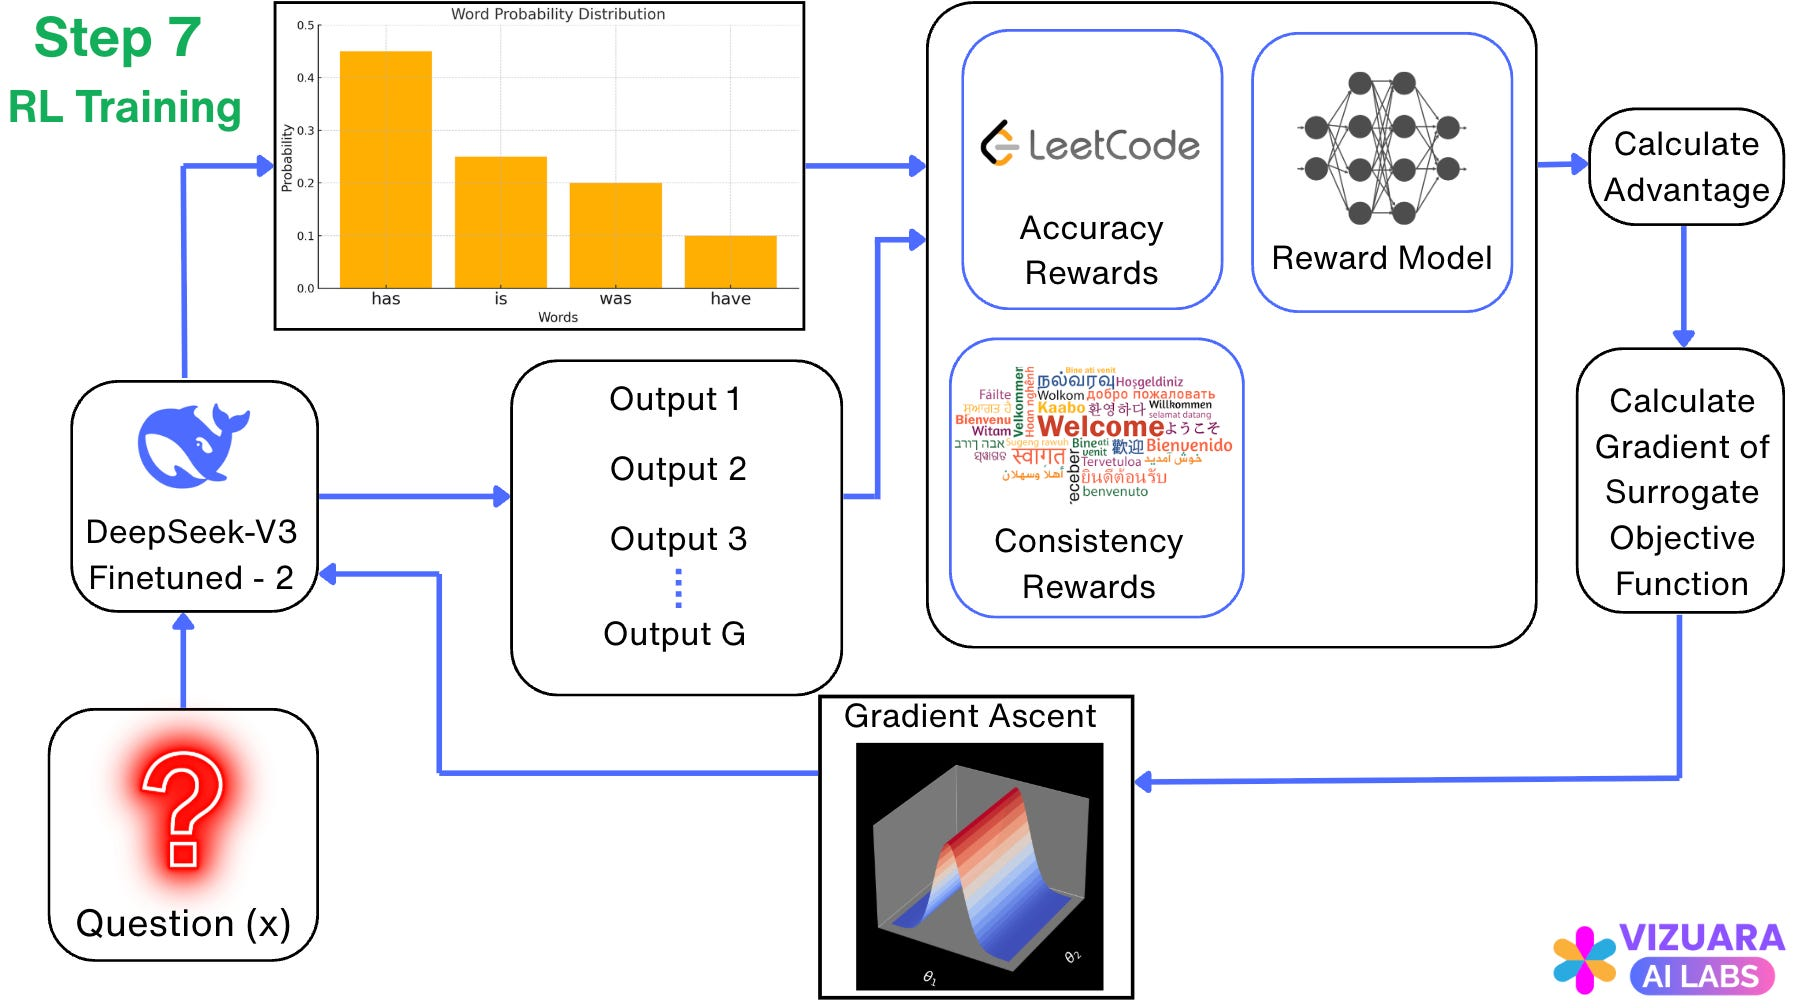
\includegraphics[width=\linewidth,keepaspectratio]{llm164}
		\end{center}

    \end{column}
    \begin{column}[T]{0.5\linewidth}
		\begin{center}
		
\includegraphics[width=0.5\linewidth,keepaspectratio]{llm165}
		\end{center}
    \end{column}
  \end{columns}
  

{\tiny (Ref: What are Large Reasoning Models? - Vizuara AI)}

\end{frame}

%%%%%%%%%%%%%%%%%%%%%%%%%%%%%%%%%%%%%%%%%%%%%%%%%%%%%%%%%%%%%%%%%%%%%%%%%%%%%%%%%%
\begin{frame}[fragile]\frametitle{Ingredient 4: Distillation}
\begin{itemize}
  \item Transfer reasoning skills to smaller models.
  \item Use large model’s outputs to train small models.
  \item Enables on-device reasoning with low memory.
  \item Example: Train Qwen 1.5B using DeepSeek-R1 data.
  \item Achieves competitive performance with tiny models.
  \item Smaller models match or outperform GPT-4o on benchmarks.
  \item Makes reasoning more accessible and efficient.
  \item Core idea: teach via imitation of a smarter model.
  \item Widely used in model compression and deployment.
\end{itemize}
\end{frame}

%%%%%%%%%%%%%%%%%%%%%%%%%%%%%%%%%%%%%%%%%%%%%%%%%%%%%%%%%%%%%%%%%%%%%%%%%%%%%%%%%%
\begin{frame}[fragile]\frametitle{Distillation}


\begin{columns}
    \begin{column}[T]{0.5\linewidth}
		\begin{center}
		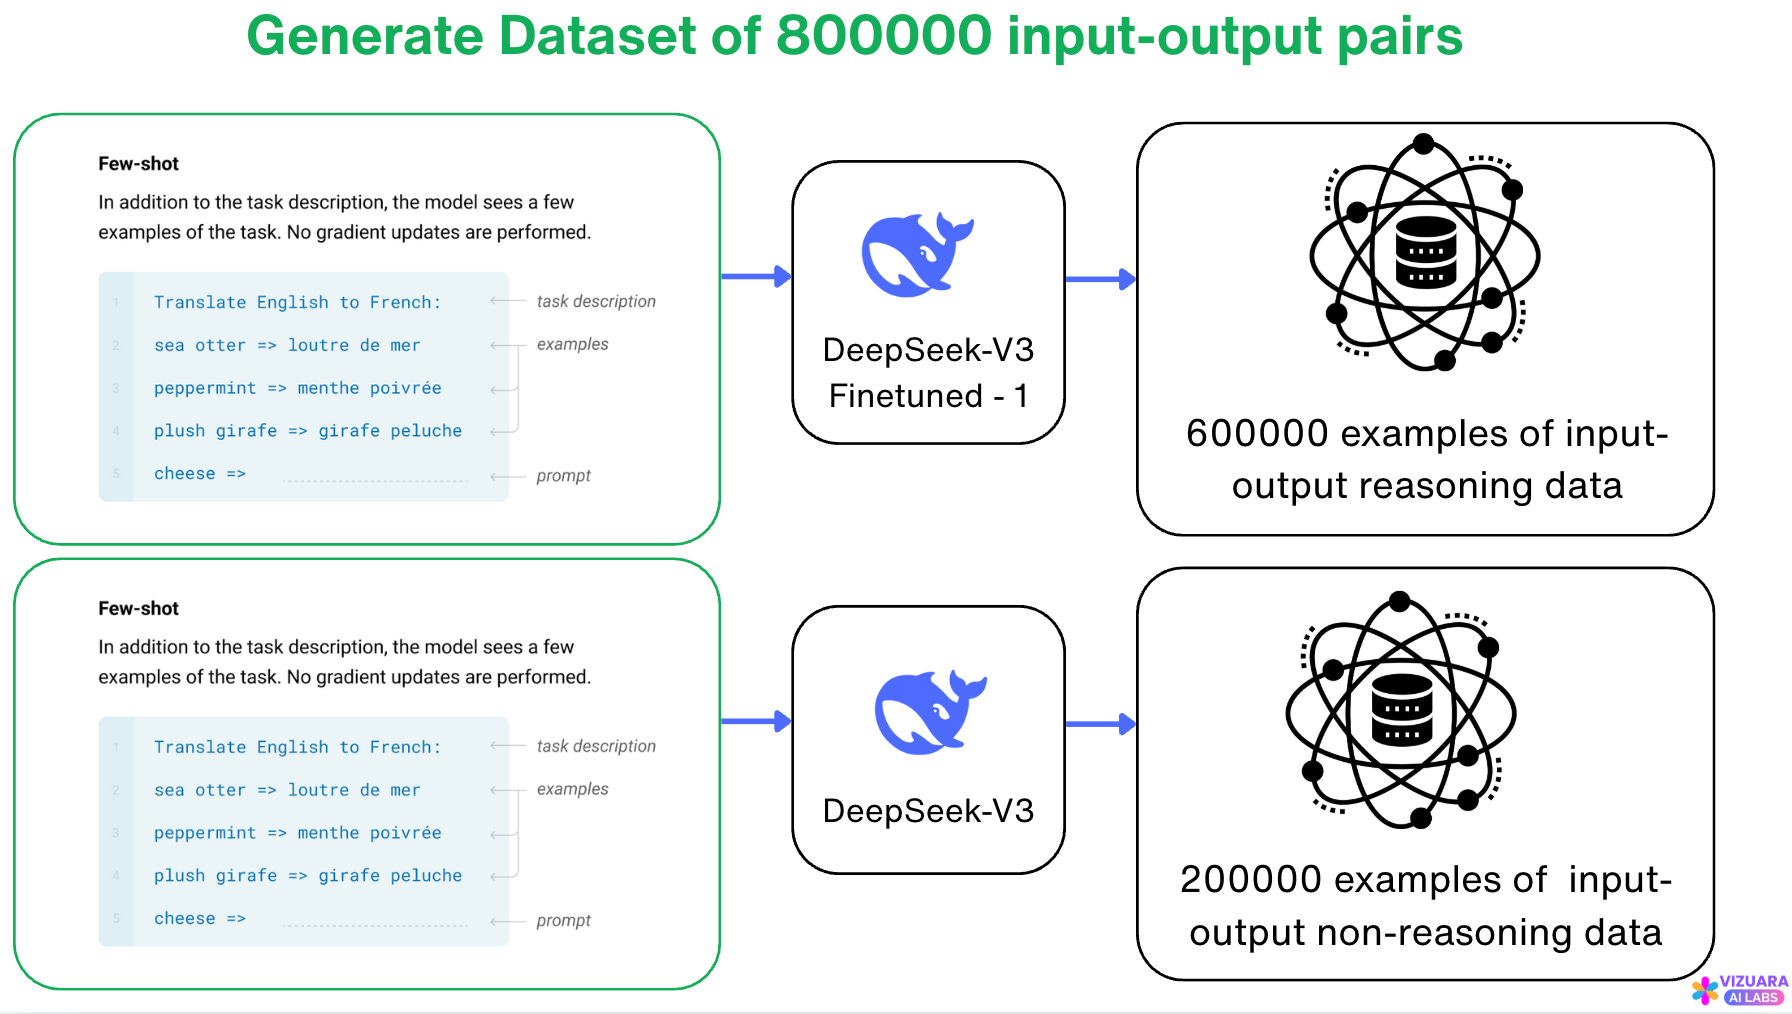
\includegraphics[width=\linewidth,keepaspectratio]{llm166}
		\end{center}

    \end{column}
    \begin{column}[T]{0.5\linewidth}
		\begin{center}
		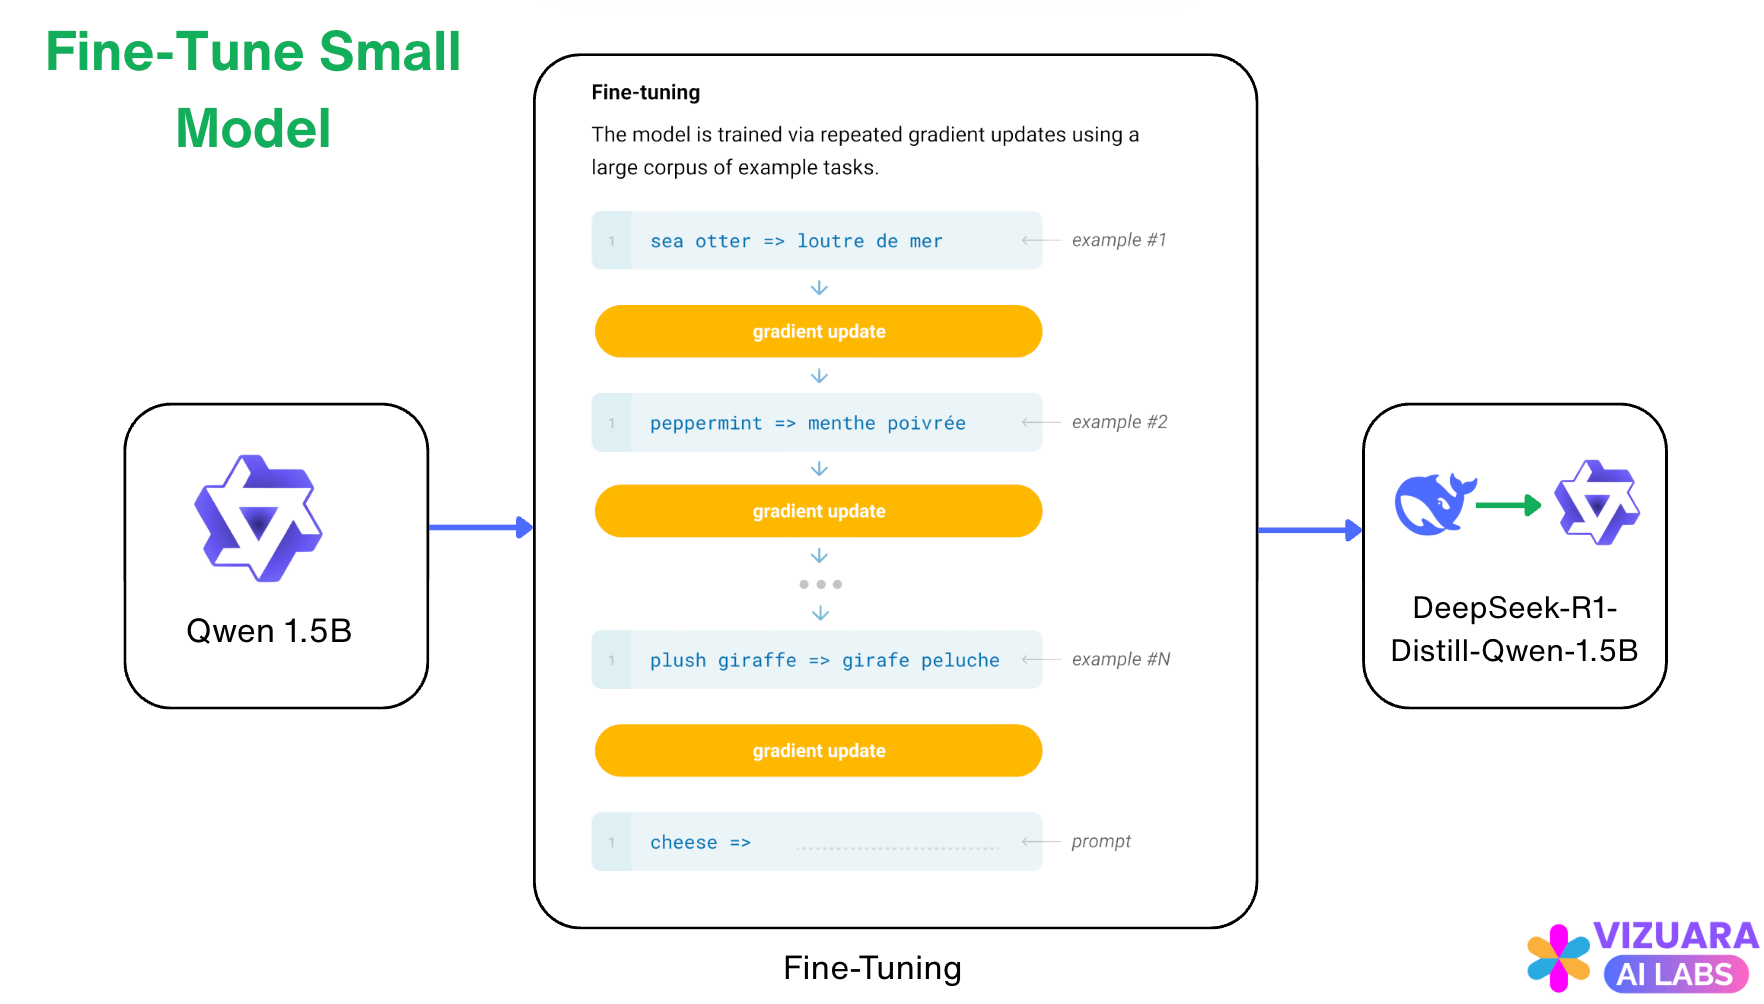
\includegraphics[width=\linewidth,keepaspectratio]{llm167}
		\end{center}
    \end{column}
  \end{columns}
  

{\tiny (Ref: What are Large Reasoning Models? - Vizuara AI)}

\end{frame}

%%%%%%%%%%%%%%%%%%%%%%%%%%%%%%%%%%%%%%%%%%%%%%%%%%%%%%%%%%%%%%%%%%%%%%%%%%%%%%%%%%
\begin{frame}[fragile]\frametitle{Final Takeaways}

\begin{columns}
    \begin{column}[T]{0.5\linewidth}
		\begin{itemize}
		  \item Reasoning distinguishes human-like intelligence.
		  \item Early LLMs lacked System 2 thinking abilities.
		  \item Four key ingredients enable reasoning in LLMs.
		  \item Inference compute boosts step-by-step thinking.
		  \item Reinforcement learning promotes exploration.
		  \item Supervised + RL fine-tuning improves generalization.
		  \item Distillation democratizes reasoning AI.
		  \item DeepSeek-R1 revealed the full recipe openly.
		  \item A new era of reasoning-capable AI has begun.
		\end{itemize}

    \end{column}
    \begin{column}[T]{0.5\linewidth}
		\begin{center}
		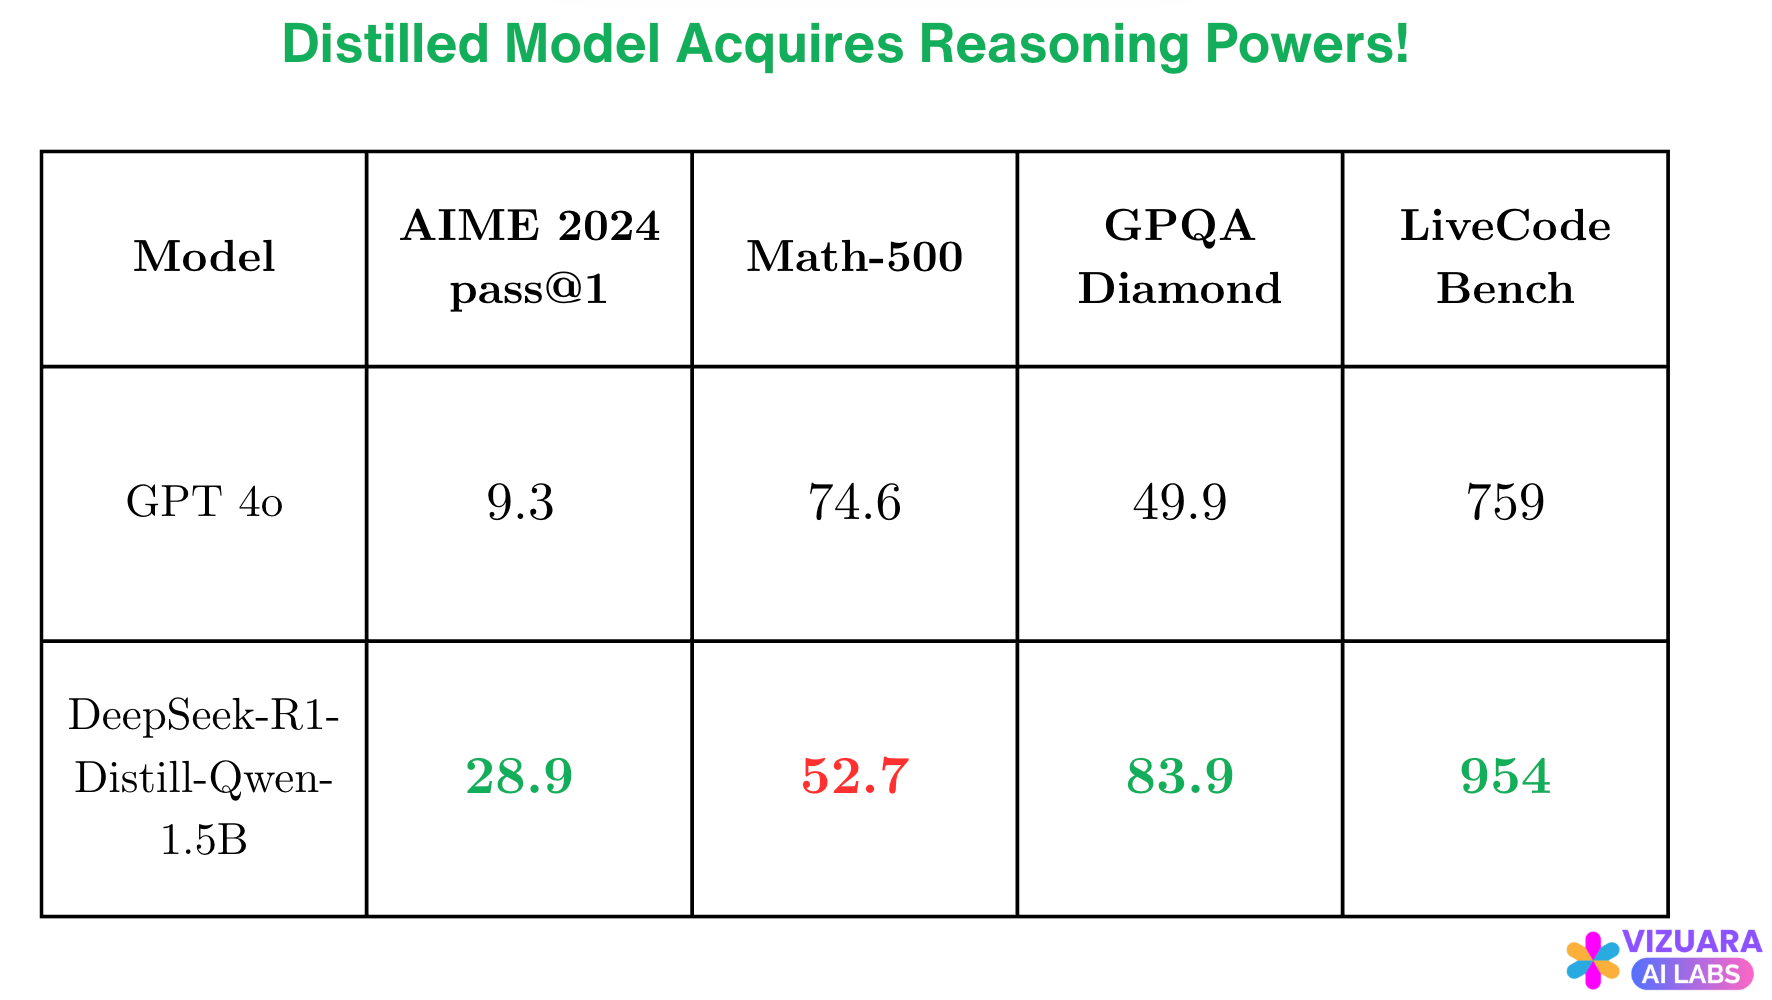
\includegraphics[width=\linewidth,keepaspectratio]{llm168}
		
		{\tiny (Ref: What are Large Reasoning Models? - Vizuara AI)}
		
		\end{center}
    \end{column}
  \end{columns}
  
\end{frame}
